% Sostituisco i placeholder registrati con la specifica variabile per il documento corrente. Questa parte iniziale contiene intestazioni e templates.

% Modificare ad ogni modifica e documento
\newcommand{\documento}{\ST}
\newcommand{\nomedocumentofisico}{SpecificaTecnica 2\_0\_0.pdf}
\newcommand{\redazione}{\MC \\ & \DAN \\ & \AN \\ & \AS \\ & \NS}
\newcommand{\verifica}{\AS}
\newcommand{\versione}{2.0.0}
\newcommand{\approvazione}{\DS}
\newcommand{\uso}{Esterno}
\newcommand{\destinateTo}{\TV, \\ & \RC, \\ & \proponente}
\newcommand{\datacreazione}{25 Febbraio 2017}
\newcommand{\datamodifica}{04 Aprile 2017}
\newcommand{\stato}{Approvato}

%Abilitazione indice delle tabelle e figure
\def\TABELLE{false}
\def\FIGURE{true}

%Inclusione di layout e variabili (Non modificare)
%Stile e dimensione del documento
\documentclass[a4paper,11pt]{article}

%Pacchetti da importare
\usepackage{ifthen}
\usepackage[italian]{babel}
\usepackage[utf8]{inputenc}
\usepackage[T1]{fontenc}
\usepackage{float}
\usepackage{chapterbib}
\usepackage{graphicx}
\usepackage[a4paper,top=2.5cm,bottom=2.5cm,left=2.5cm,right=2.5cm]{geometry}
\usepackage[colorlinks=true, urlcolor=black, citecolor=black, linkcolor=black]{hyperref}
\usepackage{booktabs}
\usepackage{fancyhdr}
\usepackage{totpages}
\usepackage{tabularx, array}
\usepackage{dcolumn}
\usepackage{epstopdf}
\usepackage{booktabs}
\usepackage{fancyhdr}
\usepackage{longtable}
\usepackage{calc}
\usepackage{datatool}
\usepackage[bottom]{footmisc}
\usepackage{listings}
\usepackage{textcomp}
\usepackage{titlesec}
\usepackage{rotating}
\usepackage{multirow}
\usepackage{placeins}
\usepackage{color}
\usepackage[table,usenames,dvipsnames]{xcolor}
\usepackage{hyperref}
\usepackage{makecell}
\usepackage{breakurl}
\usepackage{hyperref}
\usepackage{multirow}
\usepackage{xcolor,colortbl}
\usepackage{afterpage}
\usepackage{mathtools}
\usepackage{verbatim} 
\usepackage[toc,page]{appendix}

%glossary code%
\usepackage[nonumberlist,xindy]{glossaries}

\newglossarystyle{myaltlistgroup}{%
	\setglossarystyle{altlistgroup}%
	\renewcommand*{\glsgroupheading}[1]{%
		
		\newpage
		\item\makebox[\linewidth]{\Large\textbf{\glsgetgrouptitle{##1}}}%
		\vspace*{-\baselineskip}%
		\item\makebox[\linewidth]{\hspace*{3cm}\hrulefill\hspace*{3cm}}%
	}%
}



%Stile fancy per il documento (Header e footer)
\pagestyle{fancy}
%Rimuovo l'indentazione
\setlength{\parindent}{0pt}

%Imposto l'intestazione
\lhead{\Large{\progetto} \\ \footnotesize{\documento}}
%Linea sotto l'intestazione
\renewcommand{\headrulewidth}{0.4pt} 

%Footer
\lfoot{\textit{\gruppoLink}\\ \footnotesize{\email}}
%Footer con numero romano per le prime pagine
\rfoot{\thepage}
\cfoot{}
%Linea sopra il footer
\renewcommand{\footrulewidth}{0.4pt}   

%Imposta il livello degli elenchi 
\setcounter{secnumdepth}{7}
\setcounter{tocdepth}{7}

%Paragrafi impostati come una sezione
\titleformat{\paragraph}{\normalfont\normalsize\bfseries}{\theparagraph}{1em}{}
\titlespacing*{\paragraph}{0pt}{3.25ex plus 1ex minus .2ex}{1.5ex plus .2ex}

\titleformat{\subparagraph}{\normalfont\normalsize\bfseries}{\thesubparagraph}{1em}{}
\titlespacing*{\subparagraph}{0pt}{3.25ex plus 1ex minus .2ex}{1.5ex plus .2ex}

\makeatletter
\newcounter{subsubparagraph}[subparagraph]
\renewcommand\thesubsubparagraph{
  \thesubparagraph.\@arabic\c@subsubparagraph}
\newcommand\subsubparagraph{
  \@startsection{subsubparagraph}
    {6}
    {\parindent}
    {3.25ex \@plus 1ex \@minus .2ex}
    {0.75em}
    {\normalfont\normalsize\bfseries}}
\newcommand\l@subsubparagraph{\@dottedtocline{6}{10em}{5.5em}} 
\newcommand{\subsubparagraphmark}[1]{}
\makeatother

\makeatletter
\newcounter{subsubsubparagraph}[subsubparagraph]
\renewcommand\thesubsubsubparagraph{
  \thesubsubparagraph.\@arabic\c@subsubsubparagraph}
\newcommand\subsubsubparagraph{
  \@startsection{subsubsubparagraph}
    {7}
    {\parindent}
    {3.25ex \@plus 1ex \@minus .2ex}
    {0.75em}
    {\normalfont\normalsize\bfseries}}
\newcommand\l@subsubsubparagraph{\@dottedtocline{7}{10em}{6.5em}}
\newcommand{\subsubsubparagraphmark}[1]{}
\makeatother

\renewcommand\appendixtocname{Appendice}
\renewcommand\appendixpagename{Appendice}
%Variabili generali
\newcommand{\progetto}{API Market}
\newcommand{\gruppo}{NetBreak}
\newcommand{\gruppoLink}{\href{https://git.io/v1Rgz}{NetBreak}}
\newcommand{\email}{netbreakswe@gmail.com}

%Variabili riguardanti i documenti
\newcommand{\AdR}{Analisi dei Requisiti}
\newcommand{\NdP}{Norme di Progetto}
\newcommand{\PdP}{Piano di Progetto}
\newcommand{\SdF}{Studio di Fattibilità}
\newcommand{\PdQ}{Piano di Qualifica}
\newcommand{\VE}{Verbale}
\newcommand{\ST}{Specifica Tecnica}
\newcommand{\DDP}{Definizione di Prodotto}
\newcommand{\MU}{Manuale Utente}
\newcommand{\G}{Glossario}
\newcommand{\LdP}{Lettera di Presentazione}

%Variabili per i membri del gruppo
\newcommand{\AS}{Andrea Scalabrin}
\newcommand{\NS}{Nicolò Scapin}
\newcommand{\AN}{Alberto Nicolè}
\newcommand{\DS}{Davide Scarparo}
\newcommand{\DAN}{Dan Serbanoiu}
\newcommand{\MC}{Marco Casagrande}

%Ruoli di progetto
\newcommand{\RdP}{Responsabile di Progetto}
\newcommand{\Res}{Responsabile}
\newcommand{\Amm}{Amministratore}
\newcommand{\Ver}{Verificatore}
\newcommand{\Prog}{Progettista}
\newcommand{\Progr}{Programmatore}
\newcommand{\Ana}{Analista}
\newcommand{\RdPs}{Responsabili di Progetto}
\newcommand{\Ress}{Responsabile}
\newcommand{\Amms}{Amministratori}
\newcommand{\Vers}{Verificatori}
\newcommand{\Progs}{Progettisti}
\newcommand{\Progrs}{Programmatori }
\newcommand{\Anas}{Analisti}

%Professori e proponente
\newcommand{\TV}{Prof. Tullio Vardanega}
\newcommand{\RC}{Prof. Riccardo Cardin}
\newcommand{\IS}{ItalianaSoftware S.r.l.}
\newcommand{\proponente}{ItalianaSoftware S.r.l.}

\newcommand{\diaryEntry}[5]{#2 & \emph{#4} & #3 & #5 & #1\\ \hline}

%Comando per una nuova riga nella tabella del changelog
\newcommand{\specialcell}[2][c]{%
	\begin{tabular}[#1]{@{}c@{}}#2\end{tabular}}

\renewcommand*\sectionmark[1]{\markboth{#1}{}}
\renewcommand*\subsectionmark[1]{\markright{#1}}

%Variabili per la fase di lavoro
\newcommand{\AR}{Analisi dei Requisiti}
\newcommand{\ARD}{Analisi dei Requisiti Dettagliata}
\newcommand{\PA}{Progettazione Architetturale}
\newcommand{\PD}{Progettazione Architetturale Dettagliata}
\newcommand{\CO}{Codifica}
\newcommand{\VV}{Verifica e Validazione}

%Variabili per le varie revisioni
\newcommand{\RR}{Revisione dei Requisiti}
\newcommand{\RP}{Revisione di Progettazione}
\newcommand{\RPMin}{Revisione di Progettazione Minima}
\newcommand{\RPMax}{Revisione di Progettazione Massima}
\newcommand{\RQ}{Revisione di Qualifica}
\newcommand{\RA}{Revisione di Accettazione}

\newcommand{\myincludegraphics}[2][]{%
	\setbox0=\hbox{\phantom{X}}%
	\vtop{
		\hbox{\phantom{X}}
		\vskip-\ht0
		\hbox{\includegraphics[#1]{#2}}}}

\renewcommand\footnoterule{\rule{\linewidth}{1pt}}

\newcommand{\nogloxy}[1]{#1} % comando da usare per evitare di metttere il mark del glossario
\newcommand{\gloxy}[1]{\emph{#1}$_G$}

\colorlet{punct}{red!60!black}
\definecolor{background}{HTML}{EEEEEE}
\definecolor{delim}{RGB}{20,105,176}
\colorlet{numb}{magenta!60!black}
\lstdefinelanguage{json}{
	basicstyle=\small\ttfamily,
	numbers=left,
	numberstyle=\scriptsize,
	stepnumber=1,
	numbersep=8pt,
	showstringspaces=false,
	breaklines=true,
	frame=lines,
	backgroundcolor=\color{background},
	literate=
	*{0}{{{\color{numb}0}}}{1}
	{1}{{{\color{numb}1}}}{1}
	{2}{{{\color{numb}2}}}{1}
	{3}{{{\color{numb}3}}}{1}
	{4}{{{\color{numb}4}}}{1}
	{5}{{{\color{numb}5}}}{1}
	{6}{{{\color{numb}6}}}{1}
	{7}{{{\color{numb}7}}}{1}
	{8}{{{\color{numb}8}}}{1}
	{9}{{{\color{numb}9}}}{1}
	{:}{{{\color{punct}{:}}}}{1}
	{,}{{{\color{punct}{,}}}}{1}
	{\{}{{{\color{delim}{\{}}}}{1}
	{\}}{{{\color{delim}{\}}}}}{1}
	{[}{{{\color{delim}{[}}}}{1}
	{]}{{{\color{delim}{]}}}}{1},
}
\lstset{language=json}
\lstset{literate=%
	{Ö}{{\"O}}1
	{Ä}{{\"A}}1
	{Ü}{{\"U}}1
	{é}{{\"s}}1
	{è}{{\"e}}1
	{à}{{\"a}}1
	{ö}{{\"o}}1
}

\newcommand{\impl}{\textcolor{Green}{Implementato}}
\newcommand{\implno}{\textcolor{Red}{Non Implementato}}
\newcommand\Tstrut{\rule{0pt}{3.2ex}}         % = `top' strut
\newcommand\Bstrut{\rule[-1.9ex]{0pt}{0pt}}   % = `bottom' strut
\definecolor{Gray}{gray}{0.85}
\usepackage[inline]{enumitem}

%Inclusione del changelog per il documento corrente

\newcommand{\modifiche}
{
	Approvazione del documento & \specialcell[t]{\AS\\\Res} & \specialcell[t]{2017-01-04\\1.0.0}
	\\
	\midrule
	Verifica del documento & \specialcell[t]{\DS \\ \AN \\\Vers} & \specialcell[t]{2016-12-13\\0.3.0}
	\\
	\midrule
	Modifiche minori sulla base della verifica & \specialcell[t]{\AS\\\Res} & \specialcell[t]{2016-12-10\\0.2.2}
	\\
	\midrule
	Modifiche alla sezione Capitolato C3 & \specialcell[t]{\NS\\\Ana} & \specialcell[t]{2016-12-08\\0.2.1}
	\\
	\midrule
	Verifica del documento & \specialcell[t]{\AN\\\Ver} & \specialcell[t]{2016-12-07\\0.2.0}
	\\
	\midrule
	Modifiche dei paragrafi sulla base della verifica & \specialcell[t]{\AS\\\Res} & \specialcell[t]{2016-12-06\\0.1.1}
	\\
	\midrule
	Verifica del documento & \specialcell[t]{\DS\\\Ver} & \specialcell[t]{2016-12-06\\0.1.0}
	\\
	\midrule
	Accorpati i documenti e modifiche minori & \specialcell[t]{\AS\\\Res} & \specialcell[t]{2016-12-05\\0.0.9}
	\\
	\midrule
	Stesura del capitolato C2 & \specialcell[t]{\MC\\\Ana} & \specialcell[t]{2016-12-03\\0.0.8}
	\\
	\midrule
	Stesura del capitolato C5 & \specialcell[t]{\AN\\\Ana} & \specialcell[t]{2016-12-03\\0.0.7}
	\\
	\midrule
	Stesura del capitolato C4 & \specialcell[t]{\DS\\\Ana} & \specialcell[t]{2016-12-03\\0.0.6}
	\\
	\midrule
	Stesura del capitolato C3 & \specialcell[t]{\NS\\\Ana} & \specialcell[t]{2016-12-03\\0.0.5}
	\\
	\midrule
	Stesura del capitolato C6 & \specialcell[t]{\DAN\\\Ana} & \specialcell[t]{2016-12-03\\0.0.4}
	\\
	\midrule	
	Stesura del capitolato C1 & \specialcell[t]{\AS\\\Ana} & \specialcell[t]{2016-12-02\\0.0.3}
	\\
	\midrule
	Stesura dell'introduzione & \specialcell[t]{\AS\\\Ana} & \specialcell[t]{2016-12-02\\0.0.2}
	\\
	\midrule
	Creato template documento & \specialcell[t]{\AS\\\Ana} & \specialcell[t]{2016-12-02\\0.0.1}
	\\	
}


%Imposto la profondità degli indici
\setcounter{secnumdepth}{8}
\setcounter{tocdepth}{8}





\begin{document}

%Inclusione del template per la homepage (Non modificare)
%Importante: Non modificare questo template
%Modificare il documento principale per cambiare le parti

\begin{center}


%Spaziatura verticale

\vspace{4em}

%Intestazione con nome del gruppo
\begin{center} 
	\begin{Huge}
		\textbf{\fontsize{15mm}{20mm}\selectfont \gruppoLink} 
	\end{Huge}
\end{center}

\begin{center}
	\begin{Large}
		\vspace{0.3em}
		\textbf{Progetto \progetto}
	\end{Large}
\end{center}

%Inclusione del logo

\includegraphics[keepaspectratio = true,width=6cm]{../../Template/img/LogoNetbreak.png}

%Prima pagina senza intestazione né piè di pagina	
\thispagestyle{empty}

%Le informazioni del documento sono ancorate a fine pagina
\vfill

%Nome del documento
\begin{Huge} \textbf{\documento} \end{Huge}

%Tabella centrale
\begin{center}
\large\textbf{Informazioni sul documento} \\ \vspace{2em}
\small
\begin{tabular}{r l}
	\textbf{Nome del documento} & \nomedocumentofisico \\
	\textbf{Data di creazione} & \datacreazione\\
	\textbf{Ultima modifica} & \datamodifica\\
	\textbf{Versione} & \versione\\
	\textbf{Stato} & \stato \\
	\textbf{Redatto da}	& \redazione\\
	\textbf{Verificato da}	& \verifica\\
	\textbf{Approvato da}	& \approvazione\\
	\textbf{Uso}  & \uso\\
	\textbf{Distribuzione} & \gruppo \\
	\textbf{Destinato a}  &  \destinateTo \\
	\textbf{Email di riferimento}  &  \email \\
\end{tabular}
\end{center}

\vspace{2em}

\normalsize
%Inclusione abstract
\textbf{Abstract\\} 
Questo documento contiene il \PdP\ relativo al prodotto \progetto\ determinato dal gruppo \gruppo.
\end{center}
\clearpage


%Registro delle modifiche e indice (Non modificare)
\pagenumbering{Roman}
\newpage
%Tabulazione per il changelog multipagina
%Utilizzare la variabile relativa alla pagina corrispondente
%Per indicare la tabella corrispondente

\begin{center}
	\Large{\textbf{Changelog}}
	\\\vspace{0.5cm}
	\normalsize
	\begin{tabularx}{\textwidth}{cXcc}
		\textbf{Versione} & \textbf{Descrizione} & \textbf{Autore e Ruolo} & \textbf{Data}\\\toprule
		\modificheuno
		\bottomrule
	\end{tabularx}
	\newpage
	\begin{tabularx}{\textwidth}{cXcc}
		\textbf{Versione} & \textbf{Descrizione} & \textbf{Autore e Ruolo} & \textbf{Data}\\\toprule
		\modifichedue
		\bottomrule
	\end{tabularx}
\end{center}

\newpage
%Inserisce il link all'indice
%\addcontentsline{toc}{section}{Indice}
\newpage
\tableofcontents
\clearpage 

%Se è stata impostata a true la variabile per la lista delle tabelle, la mostra
\ifthenelse{\equal{\TABELLE}{true}} 
{\listoftables \newpage}{}

%Se è stata impostata a true la variabile per la lista delle figure, la mostra
\ifthenelse{\equal{\FIGURE}{true}}
{\listoffigures \newpage}{}

%Da qui comincia la numerazione normale
\pagenumbering{arabic}

%Imposta il formato di visualizzazione
\rfoot{\thepage~di~\pageref{TotPages}}

%Inclusione delle varie sezioni di contenuto
%Introduzione e contenuti di ogni tipo

\newpage
\section{Introduzione}

\subsection{Scopo del documento}
Lo scopo del documento è quello di presentare una breve analisi di tutti i capitolati proposti, con le motivazioni che hanno portato il gruppo a scegliere il capitolato C1. Tutti i capitolati son stati analizzati con la medesima metodologia,  evidenziando le tecnologie necessarie, il dominio applicativo e le criticità, e dando un giudizio finale con le opinioni raccolte all'interno del gruppo.

\subsection{Scopo del prodotto}
Lo scopo del prodotto è la realizzazione di un \textit{API Market\ped{G}} per l'acquisto e la vendita di \textit{microservizi\ped{G}}. Il sistema offrirà la possibilità di registrare nuove \textit{API\ped{G}} per la vendita, permetterà la consultazione e la ricerca di API ai potenziali acquirenti, gestendo i permessi di accesso ed utilizzo tramite creazione e controllo di relative \textit{API key\ped{G}}. Il sistema, oltre alla web app stessa, sarà corredato di un \textit{API Gateway\ped{G}} per la gestione delle richieste e il controllo delle chiavi, e fornirà funzionalità avanzate di statistiche per il gestore della piattaforma e per i fornitori dei microservizi.

\subsection{Riferimenti normativi}
\begin{itemize}
	\item \textsc{NormeDiProgetto 2\_0\_0.pdf}
\end{itemize}

\subsection{Riferimenti informativi}
\begin{itemize}
	\item \textbf{Capitolato d'appalto C1:} APIM: An API Market Platform \\ \url{http://www.math.unipd.it/~tullio/IS-1/2016/Progetto/C1.pdf}
	\item \textbf{Capitolato d'appalto C2:} AtAVi: Accoglienza tramite Assistente Virtuale \\ \url{http://www.math.unipd.it/~tullio/IS-1/2016/Progetto/C2.pdf}
	\item \textbf{Capitolato d'appalto C3:} DeGeOP: A Designer and Geo-localizer Web App for Organizational Plants \\
	\url{http://www.math.unipd.it/~tullio/IS-1/2016/Progetto/C3.pdf}
	\item \textbf{Capitolato d'appalto C4:} eBread: applicazione di lettura per dislessici \\
	\url{http://www.math.unipd.it/~tullio/IS-1/2016/Progetto/C4.pdf}
	\item \textbf{Capitolato d'appalto C5:} Monolith: an interactive bubble provider \\
	\url{http://www.math.unipd.it/~tullio/IS-1/2016/Progetto/C5.pdf}
	\item \textbf{Capitolato d'appalto C6:} SWEDesigner: editor di diagrammi UML con generazione di codice \\
	\url{http://www.math.unipd.it/~tullio/IS-1/2016/Progetto/C6.pdf}
\end{itemize}

\subsection{Glossario}
Per semplificare la consultazione e disambiguare alcune terminologie tecniche, le voci indicate con la lettera \textit{G} a pedice sono descritte approfonditamente nel documento \textsc{Glossario 2\_0\_0.pdf} e specificate solo alla prima occorrenza all'interno del suddetto documento.
\newpage
\section{Specifica del prodotto}
In questa sezione verrà descritta in maniera macroscopica l'architettura che verrà adottata durante l'attività di Progettazione. Per semplificare la comprensione, verrà utilizzato un approccio top-down, partendo dalle linee generali, fino a giungere ad una descrizione in dettaglio delle componenti.

\subsection{Architettura generale}
Il software API Market si caratterizza dalle comuni applicazioni per l'approccio a microservizi adottato nell'implementazione. In maniera differente da un applicazione monolitica, ogni componente viene realizzato come microservizio a sè stante. L'aggregazione di questi microservizi definisce l'applicazione finale e ne realizza il comportamento definitivo. Esulando dall'approccio a microservizi, il sistema sarà realizzato al pari di una classica applicazione \textit{Client-Server}, dove il lato \textit{front-end\ped{G}} (Client) si occuperà di fornire all'utente finale l'interfaccia web su cui poter interagire, mentre il lato \textit{back-end\ped{G}} (Server) gestirà e salverà i dati, e si occuperà della gestione delle chiamate API (tramite l'opportuna componente \textit{API Gateway}). La base di dati utilizzata, si occupa della raccolta di dati sensibili dell'utenza, della gestione delle applicazioni e delle chiavi e, infine, della gestione dei dati statistici.

Il sistema verrà realizzato, per il lato back-end, tramite microservizi con interfaccia Jolie, che verranno implementati con codice \textit{Java\ped{G}}. Questo approccio, sebbene la tematica sia di recente sviluppo, risulta molto gettonato dalle grandi realtà che recentemente hanno deciso di affacciarsi a questa realtà (come ad esempio l'\textit{AWS\ped{G}} Service Registry \textit{Eureka}, usato dalla piattaforma Netflix). Il lato front-end, invece, verrà implementato tramite \textit{HTML\ped{G}} e \textit{JavaScript\ped{G}}, in particolare, l'utilizzo del framework full-stack \textit{MeteorJS\ped{G}} consentirà un binding in real-time per la rappresentazione delle informazioni.
Nella realizzazione dell'API Market richiesto, verrà utilizzato il desing pattern architetturale \textbf{\textit{Model View ViewModel}}. Alcune componenti di questo pattern adotteranno un design pattern a microservizi, espresso in due varianti: a catena (\textit{Chain}) e di aggregazione (\textit{Aggregator}).
\begin{figure}[H]
	\centering
	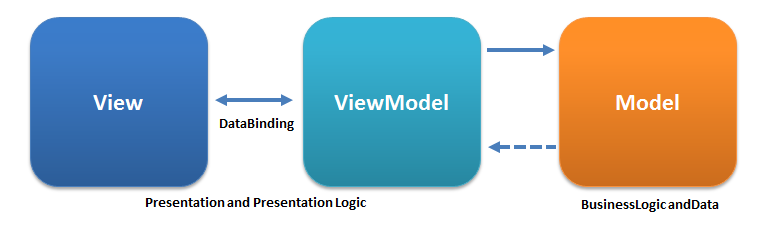
\includegraphics[width=0.7\linewidth]{IMG/MVVMPattern}
	\caption{Il design pattern Model View ViewModel}
\end{figure}

\subsubsection{Pattern architetturale front-end}
Il design pattern \textit{Model View ViewModel} (MVVM) è suddiviso in tre componenti, ed in questa sezione verranno spiegate brevemente la funzionalità di ognuna. Verrà motivata, inoltre, la scelta di tale pattern da parte del team.

\begin{itemize}
	\item \textbf{Model}: rappresenta il punto di accesso ai dati, si occupa dell'interazione con essi e ne specifica le modalità di accesso. Nella definizione dell'API Market, il Model si trova nel back-end;
	\item \textbf{View}: è in grado di gestire eventi, eseguire operazioni ed effettuare il data-binding;
	\item \textbf{ViewModel}: è il punto di incontro tra la View e il Model. I dati ricevuti da quest’ultimo sono elaborati per essere presentati e passati alla View.
\end{itemize}

In fase di progettazione, il gruppo ha preso in esame diversi design pattern architetturali, ma la volontà di realizzare pagine web dinamiche e reattive, unitamente all'uso di tecnologie moderne, quali AngularJS e il sistema di comunicazione MeteorJS, hanno indirizzato la scelta verso il pattern MVVM.

\paragraph{Componente Model}
Il Model è situato nella parte back-end del sistema e svolge le seguenti funzioni:
\begin{itemize}
	\item Interagisce con i database, nei quali vengono salvati i dati del sistema, come API, transazioni e profili utenti. Le funzionalità incluse comprendono microservizi in grado di caricare, salvare, modificare e cancellare dati sui database;
	\item Offre un'interfaccia logica di accesso al ViewModel, attraverso la quale può richiedere dati ed effettuare operazioni su di essi, tramite funzionalità del framework MeteorJS, come \textit{Publishing} e \textit{Subscribing}.
\end{itemize}

\paragraph{Componente View}
La componente View è situata nella parte front-end del sistema e ha lo scopo di:
\begin{itemize}
	\item Rappresentare i dati del ViewModel (non interagisce in nessun modo con essi);
	\item Visualizzare le funzionalità offerte all'utente.
\end{itemize} 
La componente View è un'interfaccia web, ed il gruppo ha scelto di utilizzare \textit{CSS3\ped{G}} e \textit{HTML5\ped{G}} per le parti statiche, mentre \textit{Angular 2\ped{G}} per le parti dinamiche. 

\paragraph{Componente ViewModel}
La componente ViewModel è situata nella parte front-end del sistema e comunica sia con la View che con il Model. Essa è l'unica componente a conoscere gli altri, realizzando un totale disaccopiamento tra View e Model. Il ViewModel ha tre compiti fondamentali, ovvero:
\begin{itemize}
	\item Realizzare il data-binding;
	\item Passare gli input della View e tradurli in azioni Model;
	\item Richiedere i dati al Model tramite la tecnica \textit{Publish-Subscribe} di MeteorJS, ed infine inviarli alla View.
\end{itemize}

\subsubsection{Pattern architetturale back-end}
All'interno della componente Model sono presenti una serie di microservizi relizzati con il design pattern \textbf{\textit{Aggregator Microservices}}. 
\begin{figure}[H]
	\centering
	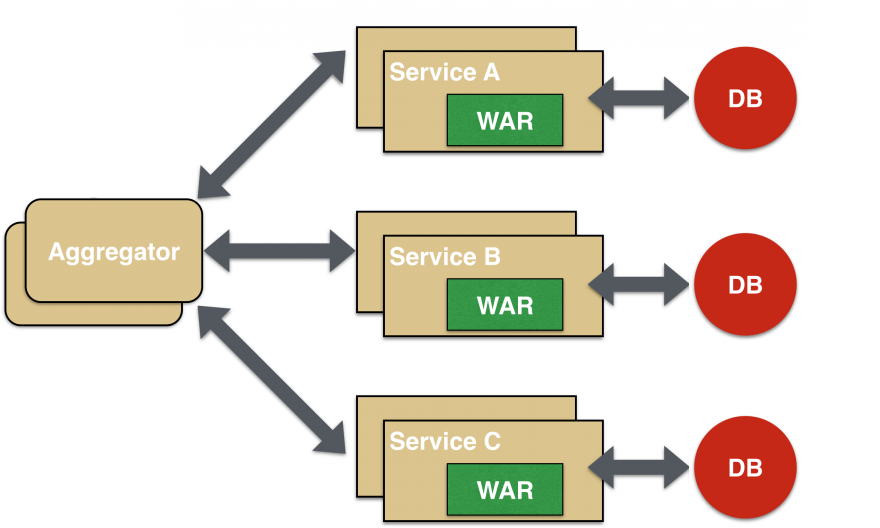
\includegraphics
	[width=0.7\linewidth]
	{IMG/microservices-aggregator}
	\caption{Aggregator Microservices design pattern}
\end{figure}
Questo design pattern si compone di un aggregatore, ovvero un microservizio in grado di collezionare i dati che gli vengono forniti da diversi microservizi, per poi renderli fruibili all'utente, tramite la componente View. Utilizzando un design pattern a microservizi è necessario che le varie componenti siano indipendenti tra loro e, quindi, che lo siano anche i relativi database. La realizzazione di un unico database avrebbe portato alla realizzazione di un'architettura \textit{SOA\ped{G}}, ovvero un'architettura orientata ai servizi, e non basata sui microservizi. Tutti i microservizi contenuti in un package, sono indipendenti da microservizi contenuti in altri package, ed ogni microservizio opera sul proprio database.

\subsubsection{Pattern architetturale API Gateway}
Il design pattern architetturale scelto per l'API Gateway è il design pattern \textbf{\textit{Chain Microservices}}. Questo tipo di pattern è una sequenza di azioni prestabilite, innescate da una richiesta \textit{HTTP\ped{G}}. 
\begin{figure}[H]
	\centering
	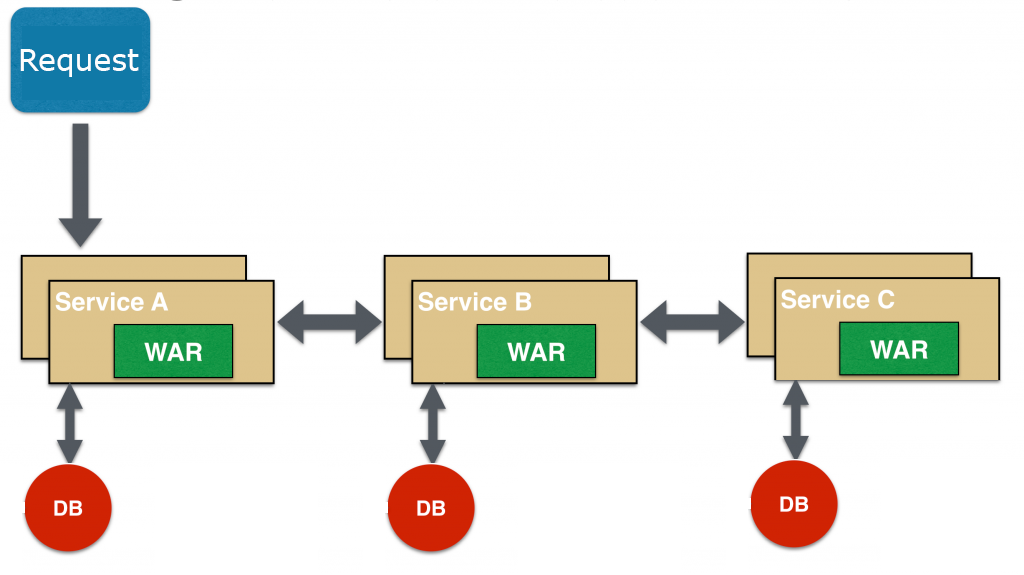
\includegraphics
	[width=0.7\linewidth]
	{IMG/microservices-chain}
	\caption{Chain Microservices design pattern}
\end{figure}
Ogni servizio non può intraprendere la propria esecuzione se non è terminato il servizio precedente. Un punto critico di questa scelta è la lunghezza della catena. L'API Gateway è progettato per elaborare una richiesta e ritornare una risposta al chiamante, trattandosi, dunque, di richieste sincrone. Una catena troppo lunga crea una tempo di attesa non indifferente per il client, considerando che bisogna valutare anche il tempo impiegato dal microservizio target della chiamata all'API Gateway.

\subsubsection{SOA vs. Microservices Architecture}
In sede di scelta architetturale, il gruppo \textit{\gruppo} ha analizzato le principali architetture in materia di microservizi. L'architettura \textbf{\textit{Service Oriented Architecture}} è una scelta intermedia tra le applicazioni monolitiche e le applicazioni completamente a microservizi. In una \textit{SOA}, l'applicazione è composta da una sorta di collezione di servizi. L'applicazione base viene, quindi, scomposta in una collezione di servizi. L’approccio a microservizi tende, invece, alla realizzazione di una singola applicazione composta da un numero arbitrario di servizi. Essi vengono, quindi, sviluppati ed implementati in maniera indipendente. Tale approccio presenta un alto livello di flessibilità e scalabilità, predisponendo la massima indipendenza dei componenti (microservizi). Un esempio è la scelta di utilizzo del database citata precedentemente: nella traduzione di un'applicazione da monolitica (oppure \textit{SOA}) ad un'architettura a microservizi, il database viene scomposto in parti indipendenti. La comunicazione tra i servizi è basata su HTTP, tramite le \textit{API RESTful\ped{G}}, con passaggio dei dati in formato \textit{JSON\ped{G}}. Nello specifico caso del nostro applicativo, la comunicazione sarà gestita su un diverso livello di astrazione, tramite i framework MeteorJS e AngularJS, i quali si occuperanno della trasmissione dati in formato JSON con maggior autonomia.

\newpage
\section{Tecnologie}
\subsection{AngularJS}
Per lo sviluppo della parte \textit{Front-End\ped{G}} dell'applicazione si è scelto di usare il \textit{framework\ped{G}} \textit{JavaScript\ped{G}} \textit{AngularJS\ped{G}}, che permette lo sviluppo di applicazioni in singola pagina. Esso consente di utilizzare HTML\ped{G} come linguaggio di template e permette di estenderne la sintassi per esprimere i componenti dell'applicazione in modo chiaro e conciso.

\subsection{Node.js}
La Web app necessita di \textit{node.js\ped{G}} per essere eseguita. Esso permette di realizzare applicazioni Web, come appunto API Market, utilizzando il linguaggio JavaScript, tipicamente client-side, per la scrittura server-side. La caratteristica principale di Node.js risiede nella possibilità che offre di accedere alle risorse del sistema operativo in modalità \textit{event-driven\ped{G}} non sfruttando il classico modello basato su processi o thread concorrenti, utilizzato dai classici web server. In particolare, si utilizzano diversi pacchetti npm dall'ecosistema Node.js quali Http-server e Bower. 

\subsection{MySQL}
MySQL o \textit{Database MySQL\ped{G}} è il più diffuso Relational Database Management system (RDBMS) composto da un client a riga di comando e un server. Entrambi i software sono disponibili sia per sistemi Unix e Unix-like che per Windows; le piattaforme principali di riferimento sono Linux e Oracle Solaris. Il software supporta numerosi applicativi per la corretta gestione dei database ad esso associato, ed è rilasciato con licenza Open Source da Oracle. 


\subsection{Jolie}
\textit{Jolie\ped{G}} è il primo linguaggio esplicitamente orientato ai microservizi. E' un linguaggio open-source utilizzato per lo sviluppo back-end a microservizi di API Market. Ogni microservizio del progetto è stato sviluppato a partire da questo linguaggio e integrato con opportune librerie Java. Jolie infatti supporta nativamente un integrazione con Java, dal quale deriva direttamente. 

\subsection{Java}
 \textit{Java\ped{G}} è un linguaggio di programmazione ad alto livello, orientato agli oggetti e a tipizzazione statica, specificatamente progettato per essere il più possibile indipendente dalla piattaforma di esecuzione. Vista la diffusione di Java e l'integrazione nativa con il linguaggio Jolie, esso si presta per l'integrazione di librerie di terze parti, quali ad esempio controlli JDBC per la connessione ai database. 
 
\subsection{Javascript}
JavaScript è un linguaggio di scripting orientato agli oggetti e agli eventi, comunemente utilizzato nella programmazione Web lato client per la creazione, in siti web e applicazioni web, di effetti dinamici interattivi tramite funzioni di script invocate da eventi innescati a loro volta in vari modi dall'utente sulla pagina web in uso (mouse, tastiera, caricamento della pagina ecc...). Tali funzioni di script possono essere opportunamente inserite in file HTML, in pagine JSP o in appositi file separati con estensione .js poi richiamati nella logica di business.

\subsection{JQuery}
\textit{jQuery\ped{G}} è una libreria JavaScript per applicazioni web. Nasce con l'obiettivo di semplificare la selezione, la manipolazione, la gestione degli eventi e l'animazione di elementi DOM in pagine HTML, nonché implementare funzionalità AJAX. 

\subsection{Bootstrap 3}
\textit{Bootstrap 3\ped{G}} è una raccolta di strumenti per la creazione di siti e applicazioni Web. Essa contiene modelli di progettazione basati su HTML e \textit{CSS\ped{G}}, sia per la tipografia, che per le varie componenti dell’interfaccia, come moduli, così come alcune estensioni opzionali di JavaScript.
\newpage
\section{Design pattern utilizzati}

\subsection{Abstract Factory}
L'\textbf{\textit{Abstract Factory}} è un design pattern creazionale e fornisce un'interfaccia per creare famiglie di prodotti, senza dover esplicitare il nome concreto delle classi a cui si riferisce. In questo modo, si permette che un sistema sia indipendente dall'implementazione degli oggetti concreti e che il client, attraverso l'interfaccia, utilizzi diverse famiglie di prodotti. Quindi, il client conosce solo l’interfaccia per creare le famiglie di prodotti, ma non la sua implementazione concreta.
L’\textit{Abstract Factory} è costituito da 5 elementi:
\begin{itemize}
	\item \textbf{AbstractFactory}: dichiara un'interfaccia per le operazioni che crea oggetti product astratti;
	\item \textbf{ConcreteFactory}: implementa le operazioni per creare oggetti concreti product di AbstractProduct. Per garantire che nel sistema esiste un’unica istanza di ciascuna ConcreteFactory, è buona norma definire ciascuna di esse come \textit{Singleton};
	\item \textbf{AbstractProduct}: interfaccia che definisce la struttura base dei product che la factory può instanziare;
	\item \textbf{ConcreteProduct}: nel sistema possono essere creati n ConcreteProduct, ciascuno dei quali dovrà implementare l’interfaccia AbstractProduct;
	\item \textbf{Client}: utilizza l’AbstractFactory per generare i prodotti concreti all’interno del sistema.
\end{itemize}

\begin{figure}[H]
	\centering
	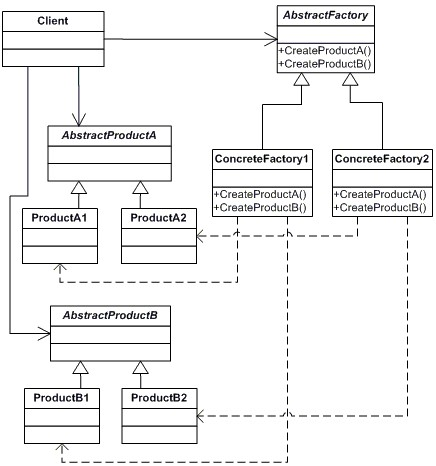
\includegraphics[width=0.5\linewidth]{IMG/abstract-pattern}
	\caption{Design pattern Abstract Factory}
\end{figure}

I punti di forza di questo design pattern sono:
\begin{itemize}
	\item Isola i client dall’implementazione delle classi concrete;
	\item Rafforza il raggruppamento di prodotti in famiglie;
	\item Rende possibile interscambiare facilmente le famiglie di prodotti, perché ogni factory concreta genera una famiglia di prodotti.
\end{itemize}

\subsubsection{Campo di utilizzo}
Nel sistema realizzato, il design pattern \textit{Abstract Factory} verrà utilizzato per rendere il sistema indipendente dalla creazione delle classi concrete ed essere aperto all’estensione tramite la definizione di nuovi tipi.


\subsection{Singleton}
Il \textbf{\textit{Singleton}} è un design pattern creazionale che ha lo scopo di garantire che venga creata una e una sola istanza di una determinata classe, e di fornire un punto di accesso globale a tale istanza.
Gli elementi caratteristici fondamentali per l'implementazione di questo pattern sono due:
\begin{itemize}
	\item Un costruttore privato, per evitare che la classe possa essere istanziata arbitrariamente;
	\item Un metodo statico per accedere alla singola istanza.
\end{itemize}
\begin{figure}[H]
	\centering
	
\includegraphics[width=0.4\linewidth]{IMG/singleton_pattern}
	\caption{Design pattern Singleton}
\end{figure}

I punti di forza di questo design pattern sono:
\begin{itemize}
	\item L'accesso controllato all'istanza;
	\item \MakeUppercase{è} possibile consentire più istanze, sempre in modo controllato.
\end{itemize}

\subsubsection{Campo di utilizzo}
Ogni servizio in AngularJS è un \textit{Singleton}, perchè ogni servizio è istanziato non più di una volta. In \progetto\ saranno presenti dei servizi per gestire le interazioni tra la web app e i database contenenti i dati.
Il design pattern \textit{Singleton} è stato utilizzato anche per il back-end della piattaforma, infatti ogni microservizio realizzato in Jolie è istanziato solo una volta all'avvio e rimane in attesa di input per operare sul database e fornire risultati al servizio chiamante del front-end. 


\subsection{Facade}
Il \textbf{\textit{Facade}} è un design pattern strutturale che permette, attraverso un'interfaccia più semplice, l'accesso a sottosistemi che espongono interfacce complesse e molto diverse tra loro, nonché a blocchi di codice complessi.
Questo rende una libreria più facile da capire, usare e testare, inoltre permette di diminuire le dipendenze tra sottosistemi senza nascondere le funzionalità di basso livello.

\begin{figure}[H]
	\centering
	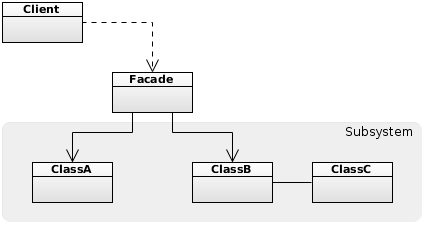
\includegraphics[width=0.7\linewidth]{IMG/facade_pattern.png}
	\caption{Design pattern Facade}
\end{figure}

I punti di forza di questo design pattern sono:
\begin{itemize}
	\item Nascondere la complessità dell'operazione all'interno di un sistema complesso;
	
	\item Fornisce un'interfaccia semplificata al client.
\end{itemize}

\subsubsection{Campo di utilizzo}
Nella parte front-end dell'applicazione, il design pattern Facade viene utilizzato nel file principale \textit{app.js}. Questo file definisce le routes dell'applicazione e viene utilizzato per associare
un URL alle varie \textit{view} dell'applicazione.\\
All'interno del file è utilizzata la funzione  \textit{\$locationProvider} e \textit{\$routeProvider} che gestiscono il routing e specificano quale pagina utilizzare in caso non venga specificato l'URL.\\
Inoltre, il pattern Facade viene utilizzato nella parte di back-end dall'API Gateway quando un utente sviluppatore inserisce un microservizio sulla piattaforma. Infatti, esso può essere composto da un numero arbitrario di interfacce e sarà compito del gateway fornire ai clienti del marketplace un'interfaccia unificata, in modo da rendere user friendly l'utilizzo.


\subsection{Decorator}
Il \textbf{\textit{Decorator}} è un design pattern strutturale che permette di aggiungere dinamicamente nuove responsabilità ad un oggetto. In questo modo, si possono estendere le funzionalità di oggetti particolari senza coinvolgere
complete classi (senza dover utilizzare il subclassing).

\begin{figure}[H]
	\centering
	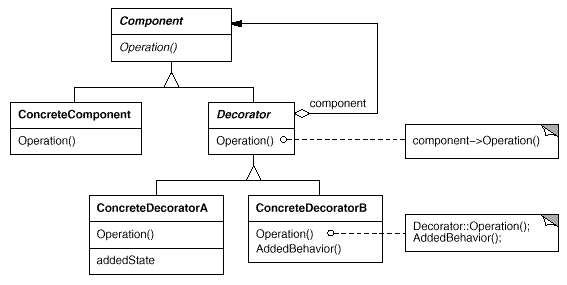
\includegraphics[width=0.7\linewidth]{IMG/decorator_pattern.png}
	\caption{Design pattern Decorator}
\end{figure}

Questa tecnica si applica quando:
\begin{itemize}
	\item Occorre aggiungere funzionalità dinamicamente ad un oggetto in modo	trasparente;
	
	\item Si vogliono "circoscrivere" le funzionalità;
	
	\item Non è possibile estendere una classe per subclassing.
\end{itemize}

\subsubsection{Campo di utilizzo}
Il pattern Decorator viene utilizzato nella parte di back-end dall'API Gateway quando avviene la richiesta di utilizzo di un microservizio da parte di un utente cliente. Il gateway deve aggiungere dinamicamente (decorare) delle informazioni alla richiesta del cliente, che ha a disposizione la sola interfaccia del microservizio target. I dati aggiunti servono per il monitoring dei dati di SLA (Service Level Agreement) e per la parte di comunicazione vera e propria con il microservizio Jolie (location e protocol).
\newpage
\section{Diagrammi dei packages e delle classi}

\subsection{Introduzione}
Questa sezione racchiude la descrizione dei diagrammi dei packages, progettati tramite un approccio top-down.\\ \textbf{N.B.: raggiunto il sub-package minimo, si procederà con la descrizione delle classi implementate al suo interno}.\\
Considerando l'approccio adottato e il particolare applicativo realizzato con un pattern a microservizi, il team non si discosterà dalla nomenclatura tradizionale di \textit{Classe}, intesa come una categoria di entità in grado di svolgere uno specifico compito. Nei diagrammi delle classi del back-end, è rappresentato graficamente come classe, ciò che in realtà è un microservizio. I suoi metodi mostrano l'interfaccia da esso esposta, mentre i campi dati saranno presenti solo nell'implementazione del microservizio.\\
Trattandosi di una progettazione con un livello di dettaglio intermedio, le classi non verranno definite, bensì verrà data una descrizione della loro funzionalità, lo scopo e le relazioni che intercorrono con le altre classi. Ogni componente individuato, quindi, verrà descritto adottando il seguente schema:
\begin{itemize}
	\item \textbf{Padre}: indica il package padre che contiene il componente in analisi;
	
	\item \textbf{Descrizione}: fornisce una breve descrizione riguardo funzionalità e scopo del componente;
	
	\item \textbf{Relazioni d'uso con altri componenti}: indica le eventuali varie relazioni d'uso con altri componenti, interne o esterna al package in analisi;
	
	\item \textbf{Package/classi contenuti/e}: elenco dei package e/o delle classi eventualmente contenuti dal componente in analisi.
\end{itemize}
L'applicativo \progetto\ è strutturato, come di consueto, in un lato front-end ed un lato back-end, come mostrato dal diagramma seguente:

\begin{figure}[H]
	\centering
	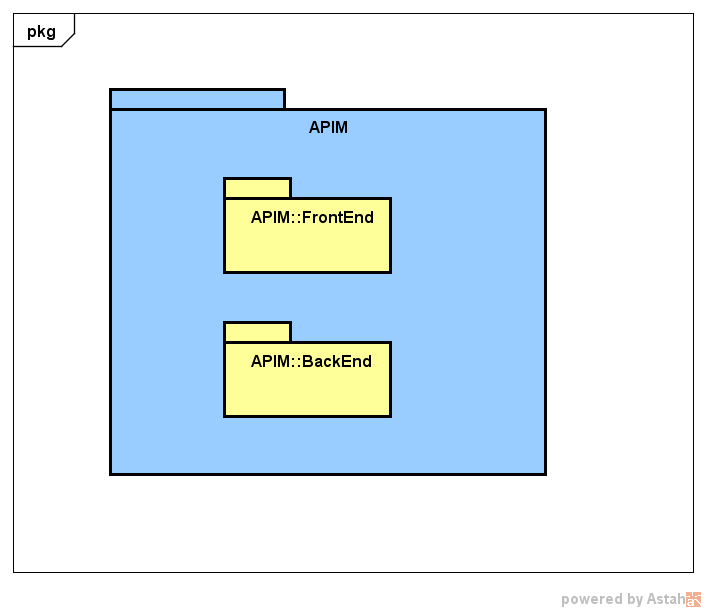
\includegraphics
	[width=0.7\linewidth]
	{UML/DiagrammiPackage/APIM.png}
	\caption{Package APIM}
\end{figure}

\newpage
\subsection{Front-end}
Nella parte front-end sono presenti i package \textit{node\_modules} e \textit{App}, che derivano dall'architettura dei componenti e framework scelti (AngularJS).

\begin{figure}[H]
	\centering
	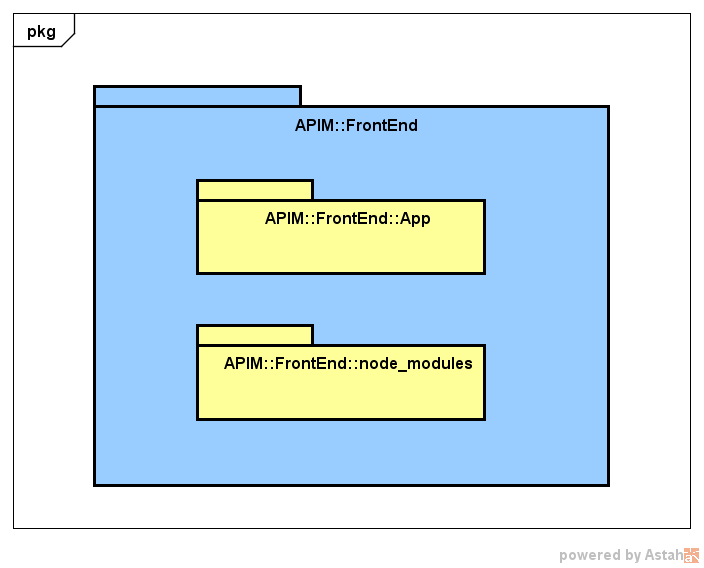
\includegraphics
	[width=0.7\linewidth]
	{UML/DiagrammiPackage/FrontEnd.png}
	\caption{Package APIM::FrontEnd}
\end{figure}

\begin{itemize}
	\item \textbf{Padre}: APIM;
	
	\item \textbf{Descrizione}: package contenente le componenti del front-end dell'applicazione;
	
	\item \textbf{Package contenuti}:
		\begin{itemize}
			\item \textbf{\textit{node\_modules}}: package contenente i riferimenti alle librerie esterne di JavaScript;
			
			\item \textbf{\textit{App}}: package contenente le componenti principali dell'applicazione.
		\end{itemize}
\end{itemize}

\subsubsection{node\_modules}
\begin{itemize}
	\item \textbf{Padre}: FrontEnd;
	
	\item \textbf{Descrizione}: package che raccoglie le librerie esterne di JavaScript, installate tramite \textit{npm} di Node.js, e fornisce le funzionalità necessarie alla parte di front-end dell'applicazione;
	
	\item \textbf{Relazioni d’uso con altri componenti}: questo package si relaziona con i \textit{controllers} presenti nel sub-package \textit{Controllers} del package \textit{App}.
\end{itemize}

\subsubsection{App}

\begin{figure}[H]
	\centering
	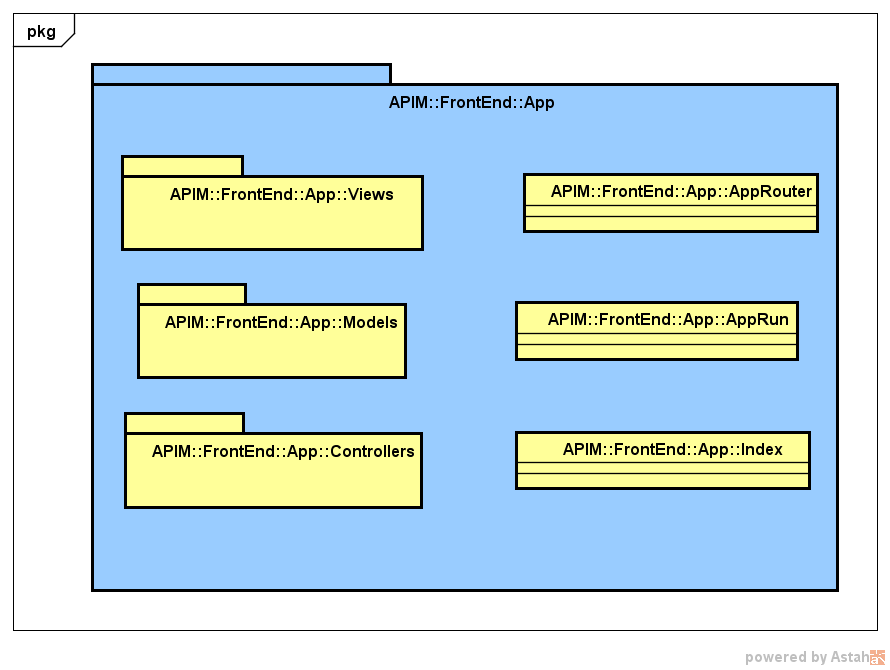
\includegraphics
	[width=0.7\linewidth]
	{UML/DiagrammiPackage/app.png}
	\caption{Package APIM::FrontEnd::App}
\end{figure}

\begin{itemize}
	\item \textbf{Padre}: FrontEnd;
	
	\item \textbf{Descrizione}: package che raccoglie le componenti principali del front-end dell'applicazione web, secondo il pattern architetturale Model-View-Controller (MVC);
	
	\item \textbf{Relazioni d’uso con altri componenti}: questo package si relaziona con le librerie presenti nel sub-package \textit{node\_modules} del package padre;
	
	\item \textbf{Package contenuti}:
		\begin{itemize}
			\item \textbf{\textit{Views}}: package contenente le \textit{views} del front-end dell'applicazione;
			
			\item \textbf{\textit{Models}}: package contenente i \textit{models} del front-end dell'applicazione;
			
			\item \textbf{\textit{Controllers}}: package contenente i \textit{controllers} del front-end dell'applicazione.
		\end{itemize}
	\item \textbf{Classi contenute}:
		\begin{itemize}
			
			\item \textbf{\textit{AppRun}}: classe che istanzia l'applicazione;
			
			\item \textbf{\textit{AppRouter}}: classe che gestisce i routes dell'applicazione;
			
			\item \textbf{\textit{Index}}: view generale dell'applicazione (single page app).
		\end{itemize}
\end{itemize}

\paragraph{AppRun}

\begin{itemize}
	\item \textbf{Padre}: App;
	
	\item \textbf{Descrizione}: classe che istanzia l'applicazione e che viene utilizzata per indicare le dipendenze tra l'applicazione e i packages esterni.
\end{itemize}

\paragraph{AppRouter}

\begin{itemize}
	\item \textbf{Padre}: App;
	
	\item \textbf{Descrizione}: classe che gestisce i routes dell'applicazione al fine di associare ad ogni route un controller e una view (associa un URL alle varie view dell'applicazione).
\end{itemize}

\paragraph{Index}

\begin{itemize}
	\item \textbf{Padre}: App;
	
	\item \textbf{Descrizione}: classe che rappresenta la view generale dell'applicazione e che contiene gli elementi che saranno presenti in ogni pagina dell'applicazione.
\end{itemize}

\paragraph{Views}

\begin{figure}[H]
	\centering
	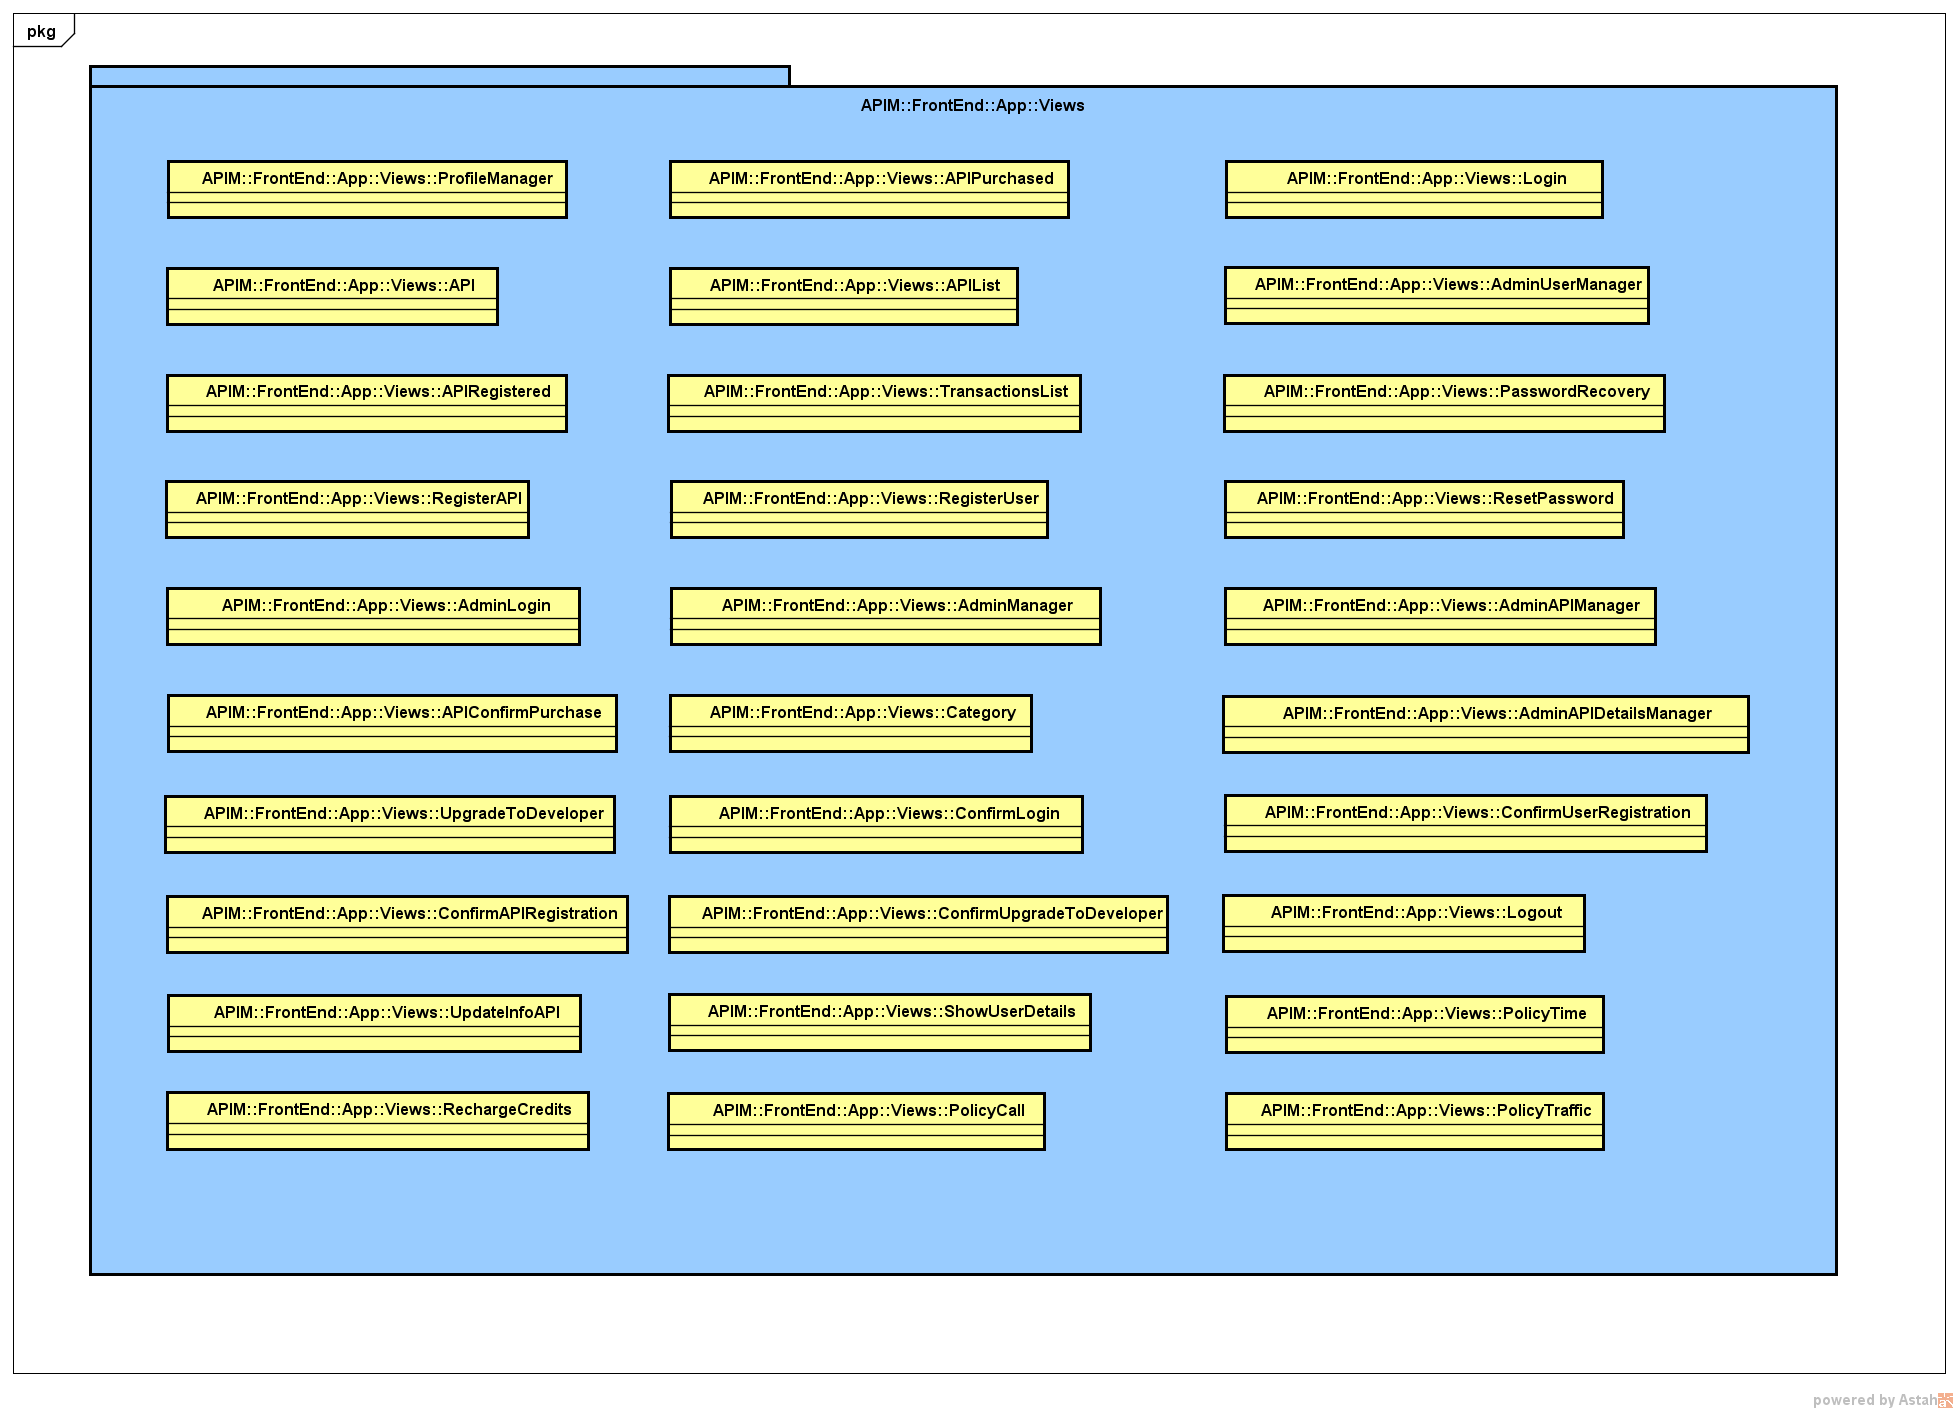
\includegraphics
	[width=0.9\linewidth]
	{UML/DiagrammiPackage/views.png}
	\caption{Package APIM::FrontEnd::App::Views}
\end{figure}

\begin{itemize}
	\item \textbf{Padre}: App;
	
	\item \textbf{Descrizione}: package contenente tutte le classi che rappresentano i vari template HTML per le pagine web dell'applicazione;
	
	\item \textbf{Relazioni d’uso con altri componenti}: questo package si relaziona con i \textit{controllers} presenti nel package \textit{Controllers};
	
	\item \textbf{Classi contenute}:
	\begin{itemize}
		\item \textbf{\textit{RegisterUser}}: view contenente il form dedicato alla registrazione di un utente, il quale può inserire i campi necessari e registrarsi così alla piattaforma. Contiene, inoltre, un link alla pagina di login.\\
		Si relaziona con le seguenti componenti: \textit{UserRegistrationController}.
		
		\item \textbf{\textit{Login}}: view contenente il form necessario affinchè l'utente possa effettuare il login ed autenticarsi al sistema. Contiene, inoltre, un link alla pagina di registrazione e uno alla pagina per il recupero della password.\\
		Si relaziona con le seguenti componenti: \textit{LoginController}.
		
		\item \textbf{\textit{PasswordRecovery}}: view contenente il form dedicato al recupero della password di un utente, il quale può inserire l'indirizzo email e ricevere una nuova password con la quale autenticarsi al sistema. Contiene, inoltre, un link alla pagina di login.\\
		Si relaziona con le seguenti componenti: \textit{PasswordRecoveryController}.
		
		\item \textbf{\textit{API}}: view contenente i risultati della ricerca effettuata, che permette di selezionare un risultato presente al suo interno.\\
		Si relaziona con le seguenti componenti: \textit{SearchController}.
		
		\item \textbf{\textit{ProfileManager}}: view contenente le informazioni del profilo personale di un utente registrato. Contiene, inoltre, l'informazione relativa al saldo del proprio conto virtuale.\\
		Si relaziona con le seguenti componenti: \textit{ProfileManagerController}.
		
		\item \textbf{\textit{ResetPassword}}: view contenente il form dedicato al cambio di password di un utente autenticato, il quale può inserire la nuova password che intende utilizzare per i futuri login al sistema.\\
		Si relaziona con le seguenti componenti: \textit{ResetPasswordController}.
		
		\item \textbf{\textit{RegisterAPI}}: view contenente il form per l'inserimento di una API da parte di un utente sviluppatore. Lo sviluppatore può inserire tutti i dati relativi al microservizio che intende esporre sul marketplace.\\
		Si relaziona con le seguenti componenti: \textit{APIRegistrationController}.
		
		\item \textbf{\textit{PolicyCall}}: view contenente le informazioni relative alla policy per chiamate.\\
		Si relaziona con le seguenti componenti: \textit{PolicyCallController}.
		
		\item \textbf{\textit{PolicyTime}}: view contenente le informazioni relative alla policy per tempo.\\
		Si relaziona con le seguenti componenti: \textit{PolicyTimeController}.
		
		\item \textbf{\textit{PolicyTraffic}}: view contenente le informazioni relative alla policy per traffico dati.\\
		Si relaziona con le seguenti componenti: \textit{PolicyTrafficController}.
		
		\item \textbf{\textit{APIRegistered}}: view contenente le informazioni di una API registrata sulla piattaforma.\\
		Si relaziona con le seguenti componenti: \textit{APIRegisteredController}.
		
		\item \textbf{\textit{APIPurchased}}: view contenente le informazioni delle API acquistate da un cliente della piattaforma \progetto.\\
		Si relaziona con le seguenti componenti: \textit{APIPurchasedController}.
		
		\item \textbf{\textit{APIList}}: view contenente l'elenco delle API disponibili sul marketplace \progetto.\\
		Si relaziona con le seguenti componenti: \textit{APIListController}.
		
		\item \textbf{\textit{TransactionsList}}: view contenente l'elenco delle transazioni effettuate da un utente sul marketplace \progetto.\\
		Si relaziona con le seguenti componenti: \textit{TransactionsListController}.
				
		\item \textbf{\textit{APIConfirmPurchase}}: view contenente la conferma di un acquisto di una API.\\
		Si relaziona con le seguenti componenti: \textit{APIConfirmPurchaseController}.
				
		\item \textbf{\textit{AdminManager}}: view contenente le operazioni per la gestione del profilo amministratore \progetto.\\
		Si relaziona con le seguenti componenti: \textit{AdminManagerController}.
		
		\item \textbf{\textit{Category}}: view contenente l'elenco delle categoria nell'\progetto.\\
		Si relaziona con le seguenti componenti: \textit{CategoryController}.
		
		\item \textbf{\textit{ConfirmUpgradeToDeveloper}}: view contenente la conferma dell'upgrade di un utente a sviluppatore nell'\progetto.\\
		Si relaziona con le seguenti componenti: \textit{ConfirmUpgradeToDeveloperController}.
		
		\item \textbf{\textit{ConfirmLogin}}: view contenente la conferma di login all'\progetto.\\
		Si relaziona con le seguenti componenti: \textit{ConfirmLoginController}.
		
		\item \textbf{\textit{ConfirmUserRegistration}}: view contenente la conferma di registrazione all'\progetto.\\
		Si relaziona con le seguenti componenti: \textit{ConfirmUserRegistrationController}.
		
		\item \textbf{\textit{ConfirmAPIRegistration}}: view contenente la conferma di registrazione di una API all'\progetto.\\
		Si relaziona con le seguenti componenti: \textit{ConfirmAPIRegistrationController}.
		
		\item \textbf{\textit{UpgradeToDeveloper}}: view contenente il modulo per diventare sviluppatore all'interno dell'\progetto.\\
		Si relaziona con le seguenti componenti: \textit{UpgradeToDeveloperController}.
		
		\item \textbf{\textit{AdminAPIManager}}: view contenente le operazioni dell'amministratore sulle API dell'\progetto.\\
		Si relaziona con le seguenti componenti: \textit{AdminAPIManagerController}.
		
		\item \textbf{\textit{AdminAPIDetailsManager}}: view contenente le statistiche di una API dell'\progetto.\\
		Si relaziona con le seguenti componenti: \textit{AdminAPIDetailsManagerController}.
		
		\item \textbf{\textit{AdminUserManager}}: view contenente le operazioni di un ammistratore sugli utenti dell'\progetto.\\
		Si relaziona con le seguenti componenti: \textit{AdminUserManagerController}.
		
		\item \textbf{\textit{AdminLogin}}: view contenente il form necessario affinchè l'amministratore possa effettuare il login ed autenticarsi al sistema.\\
		Si relaziona con le seguenti componenti: \textit{AdminLoginController}.
		
		\item \textbf{\textit{Logout}}: view contenente la conferma di logout dall'\progetto.\\
		Si relaziona con le seguenti componenti: \textit{LogoutController}.
		
		\item \textbf{\textit{UpdateInfoAPI}}: view contenente il form dedicato modifica delle informazioni di una API presente nel marketplace \progetto.\\
		Si relaziona con le seguenti componenti: \textit{UpdateInfoAPIController}.
		
		\item \textbf{\textit{RechargeCredits}}: view contenente la possibilità di scegliere quanti crediti ricaricare sul conto personale tra i tagli disponibili.\\
		Si relaziona con le seguenti componenti: \textit{RechargeCreditsController}.
		
		item \textbf{\textit{ShowUserDetalis}}: view contenente le informazioni personali di un utente visualizzabili da altri fruitori del marketplace \progetto.\\
		Si relaziona con le seguenti componenti: \textit{ShowUserDetalisController}.
		
		\item \textbf{\textit{AdminModeration}}: view contenente il form dedicato alla moderazione di un utente o di una API/microservizio da parte di un amministratore della piattaforma \progetto.\\
		Si relaziona con le seguenti componenti: \textit{AdminModerationController}.
	\end{itemize}
\end{itemize}

\paragraph{Models}

\begin{figure}[H]
	\centering
	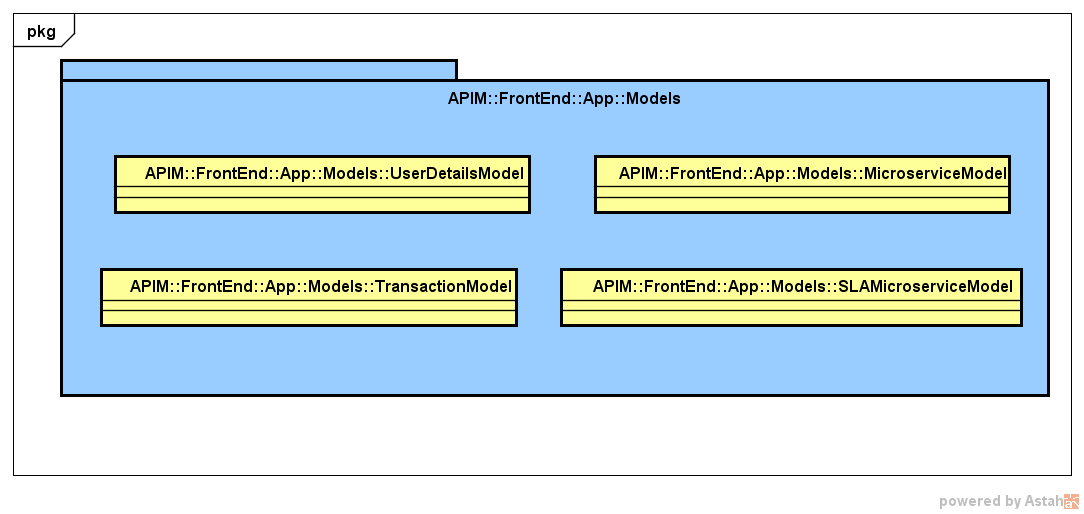
\includegraphics
	[width=0.7\linewidth]
	{UML/DiagrammiPackage/Models.png}
	\caption{Package APIM::FrontEnd::App::Models}
\end{figure}

\begin{itemize}
	\item \textbf{Padre}: App;
	
	\item \textbf{Descrizione}: package che contiene le classi che definiscono la business logic dell'applicazione;
	
	\item \textbf{Relazioni d’uso con altri componenti}: questo package si relaziona con il package \textit{Controllers};
	
	\item \textbf{Classi contenute}:
	\begin{itemize}
		\item \textbf{\textit{UserDetailsModel}}: classe che rappresenta un utente e che contiene tutte le informazioni necessarie alla presentazione del contenuto di un utente, sia nella visualizzazione che nella gestione di un profilo.\\
		Si relaziona con le seguenti componenti: \textit{LoginController}, \textit{SearchController}, \textit{ProfileManagerController}, \textit{ResetPasswordController}, \textit{PasswordRecoveryController}.
		
		\item \textbf{\textit{MicroserviceModel}}: classe che rappresenta un microservizio e che contiene tutte le informazioni necessarie alla presentazione del contenuto di un microservizio, sia nella visualizzazione che nella gestione.\\
		Si relaziona con le seguenti componenti: \textit{APIRegiteredController}, \textit{APIRegistrationController}, \textit{PolicyCall}, \textit{PolicyTime}, \textit{PolicyTraffic}, \textit{APIPurchasedController}, \textit{APIListController}.
		
		\item \textbf{\textit{TransactionModel}}:  classe che rappresenta una transazione avvenuta e che contiene tutte le informazioni necessarie alla presentazione del contenuto di una transazione, sia nella visualizzazione che nella gestione.\\
		Si relaziona con le seguenti componenti: \textit{TransactionsListController}, \textit{APIPurchasedController}.
		
		\item \textbf{\textit{SLAMicroserviceModel}}:  classe che rappresenta la SLA di un microservizio e che contiene tutte le informazioni necessarie alla presentazione del contenuto di SLA di un microservizio, sia nella visualizzazione che nella gestione.\\
		Si relaziona con le seguenti componenti: \textit{PolicyCall}, \textit{PolicyTime}, \textit{PolicyTraffic}, \textit{APIRegistrationController}.
	\end{itemize}
\end{itemize}
	
\paragraph{Controllers}

\begin{figure}[H]
	\centering
	\includegraphics
	[width=0.9\linewidth]
	{UML/DiagrammiPackage/controllers.png}
	\caption{Package APIM::FrontEnd::App::Controllers}
\end{figure}

\begin{itemize}
	\item \textbf{Padre}: App;
	
	\item \textbf{Descrizione}: package che contiene i \textit{controllers} individuati per la parte front-end
	dell'applicazione, i quali consentono la gestione delle azioni utente dell'applicazione web;
	
	\item \textbf{Relazioni d’uso con altri componenti}: questo package si relaziona con i package \textit{Views} e \textit{Models}.
	
	\item \textbf{Classi contenute}:
	\begin{itemize}
		
		\item \textbf{\textit{UserRegistrationController}}: classe che permette di gestire la registrazione di un utente al sistema, fornendone le funzionalità preposte.\\
		Si relaziona con le seguenti componenti: \textit{RegisterUser}.
		
		\item \textbf{\textit{LoginController}}: classe che permette di gestire il login di un utente alla piattaforma \progetto, fornendo le funzionalità di autenticazione al sistema, compresa la gestione di	situazioni di errore di autenticazione.\\
		Si relaziona con le seguenti componenti: \textit{UserDetailsModel}, \textit{Login}.
		
		\item \textbf{\textit{PasswordRecoveryController}}: classe che permette di gestire il ripristino della password dimenticata da un utente, fornendo tutte le funzionalità per il recupero della password dopo aver verificato l'identità dell'utente.\\
		Si relaziona con le seguenti componenti: \textit{UserDetailsModel}, \textit{PasswordRecovery}.
		
		\item \textbf{\textit{SearchController}}: classe che permette di gestire la ricerca di microservizi all'interno del marketplace \progetto, fornendo all'utente le funzionalità di ricerca tramite categorie e keywords per sviluppatori e microservizi.\\
		Si relaziona con le seguenti componenti: \textit{API}.
		
		\item \textbf{\textit{ProfileManagerController}}: classe che permette di gestire il profilo personale di un utente, fornendo le funzionalità all'utente per poter modificare i propri dati.\\
		Si relaziona con le seguenti componenti: \textit{UserDetailsModel}, \textit{ProfileManager}.
		
		\item \textbf{\textit{ResetPasswordController}}: classe che permette di gestire il cambio password di un utente autenticato al sistema, fornendo le funzionalità per il salvataggio di una nuova password.\\
		Si relaziona con le seguenti componenti: \textit{UserDetailsModel}, \textit{ResetPassword}.
		
		\item \textbf{\textit{APIRegistrationController}}: classe che permette di gestire l'inserimento di una API, fornendo tutte le funzionalità atte alla corretta esposizione di un microservizio di uno sviluppatore, utente della piattaforma \progetto.\\
		Si relaziona con le seguenti componenti: \textit{MicroserviceModel}, \textit{RegisterAPI}.
				
		\item \textbf{\textit{PolicyCallController}}: classe che permette di gestire le policy di vendita dei microservizi per chiamate.\\
		Si relaziona con le seguenti componenti: \textit{PolicyCall}, \textit{SLAMicroserviceModel}.
		
		\item \textbf{\textit{PolicyTimeController}}: classe che permette di gestire le policy di vendita dei microservizi per tempo.\\
		Si relaziona con le seguenti componenti: \textit{PolicyTime}, \textit{SLAMicroserviceModel}.
		
		\item \textbf{\textit{PolicyTrafficController}}: classe che permette di gestire le policy di vendita dei microservizi per traffico dati.\\
		Si relaziona con le seguenti componenti: \textit{PolicyTraffic}, \textit{SLAMicroserviceModel}.
		
		\item \textbf{\textit{APIRegisteredController}}: classe che permette di gestire le informazioni di una API precedentemente inserita.\\
		Si relaziona con le seguenti componenti: \textit{MicroserviceModel}, \textit{APIRegistered}.
		
		\item \textbf{\textit{APIPurchasedController}}: classe che permette di gestire l'acquisto e le relative informazioni di una API, fornendo l'API Key per l'utilizzo del cliente.\\
		Si relaziona con le seguenti componenti: \textit{APIPurchased}, \textit{MicroserviceModel}, \textit{TransactionModel}.
		
		\item \textbf{\textit{APIListController}}: classe che permette di gestire l'elenco dei microservizi presenti sul marketplace \progetto.\\
		Si relaziona con le seguenti componenti: \textit{APIList}, \textit{MicroserviceModel}.
		
		\item \textbf{\textit{TransactionsListController}}: classe che permette di gestire lo storico delle transazioni di un utente del marketplace \progetto.\\
		Si relaziona con le seguenti componenti: \textit{TransactionsList}, \textit{TransactionsModel}.
			
		\item \textbf{\textit{AdminManagerController}}: classe che permette di gestire il profilo di un amministratore della piattaforma \progetto, fornendo le funzionalità per poter modificare i propri dati e moderare utenti ed API.\\
		Si relaziona con le seguenti componenti: \textit{AdminManager}.
		%----------------------
		
		\item \textbf{\textit{CategoryController}}: classe che permette di gestire l'elenco delle categoria nell'\progetto.\\
		Si relaziona con le seguenti componenti: \textit{Category}.
		
		\item \textbf{\textit{ConfirmUpgradeToDeveloperController}}: classe che permette di gestire la conferma dell'upgrade di un utente a sviluppatore nell'\progetto.\\
		Si relaziona con le seguenti componenti: \textit{ConfirmUpgradeToDeveloper}.
		
		\item \textbf{\textit{ConfirmLoginController}}: classe che permette di gestire la conferma di login all'\progetto.\\
		Si relaziona con le seguenti componenti: \textit{ConfirmLogin}.
		
		\item \textbf{\textit{ConfirmUserRegistrationController}}: classe che permette di gestire la conferma di registrazione all'\progetto.\\
		Si relaziona con le seguenti componenti: \textit{ConfirmUserRegistration}.
		
		\item \textbf{\textit{ConfirmAPIRegistrationController}}: classe che permette di gestire la conferma di registrazione di una API all'\progetto.\\
		Si relaziona con le seguenti componenti: \textit{ConfirmAPIRegistration}.
		
		\item \textbf{\textit{UpgradeToDeveloperController}}: classe che permette di gestire il modulo per diventare sviluppatore all'interno dell'\progetto.\\
		Si relaziona con le seguenti componenti: \textit{UpgradeToDeveloper}.
		
		\item \textbf{\textit{AdminAPIManagerController}}: classe che permette di gestire le operazioni dell'amministratore sulle API dell'\progetto.\\
		Si relaziona con le seguenti componenti: \textit{AdminAPIManager}.
		
		\item \textbf{\textit{AdminAPIDetailsManagerController}}: classe che permette di gestire le statistiche di una API dell'\progetto.\\
		Si relaziona con le seguenti componenti: \textit{AdminAPIDetailsManager}.
		
		\item \textbf{\textit{AdminUserManagerController}}: classe che permette di gestire le operazioni di un ammistratore sugli utenti dell'\progetto.\\
		Si relaziona con le seguenti componenti: \textit{AdminUserManager}.
		
		\item \textbf{\textit{AdminLoginController}}: classe che permette di gestire il form necessario affinchè l'amministratore possa effettuare il login ed autenticarsi al sistema.\\
		Si relaziona con le seguenti componenti: \textit{AdminLogin}.
		
		\item \textbf{\textit{Logout}}: classe che permette di gestire la conferma di logout dall'\progetto.\\
		Si relaziona con le seguenti componenti: \textit{LogoutController}.
		
		\item \textbf{\textit{UpdateInfoAPIController}}: classe che permette di gestire il form dedicato modifica delle informazioni di una API presente nel marketplace \progetto.\\
		Si relaziona con le seguenti componenti: \textit{UpdateInfoAPI}.
		
		\item \textbf{\textit{RechargeCreditsController}}: classe che permette di gestire la possibilità di scegliere quanti crediti ricaricare sul conto personale tra i tagli disponibili.\\
		Si relaziona con le seguenti componenti: \textit{RechargeCredits}.
		
		item \textbf{\textit{ShowUserDetalisController}}: classe che permette di gestire le informazioni personali di un utente visualizzabili da altri fruitori del marketplace \progetto.\\
		Si relaziona con le seguenti componenti: \textit{ShowUserDetalis}
		
		
		%---------------------
		
		\item \textbf{\textit{AdminModerationController}}: classe che permette di gestire la moderazione di un utente (cliente o sviluppatore che sia) e di API, fornendo le funzionalità per la sospensione e rimozione.\\
		Si relaziona con le seguenti componenti: \textit{AdminModeration}.
		
	\end{itemize}
\end{itemize}
\newpage
\subsection{Back-end}

Nella parte back-end sono presenti i package \textit{Gateway} e \textit{Services} strutturati secondo un'architettura a microservizi, i quali hanno una dipendenza verso l'interfaccia \textit{serviceInteractionHandler}.

\begin{figure}[H]
	\centering
	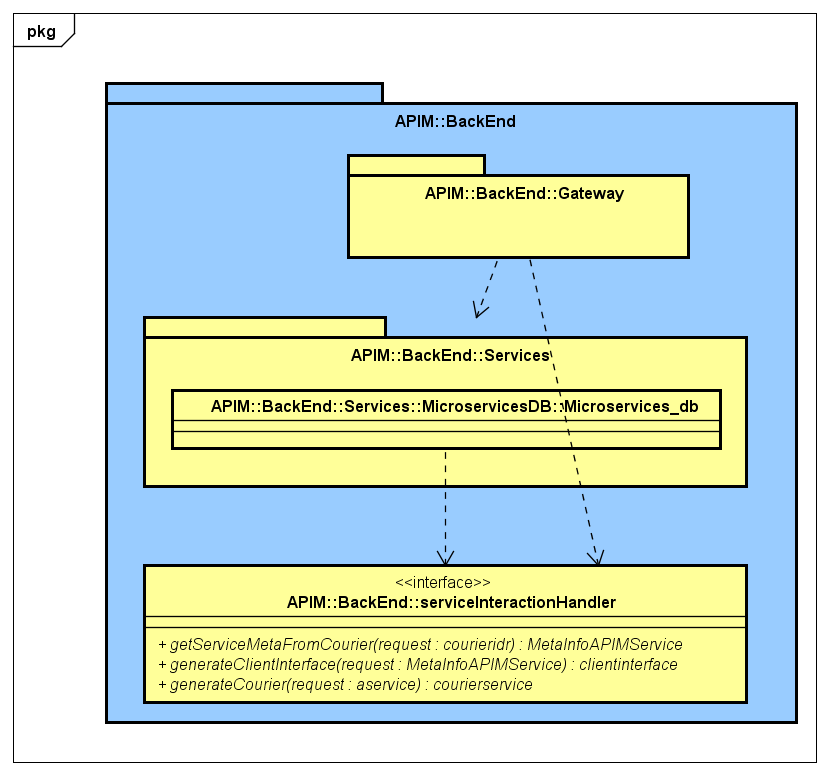
\includegraphics
	[width=0.7\linewidth]
	{UML/DiagrammiPackage/BackEnd.png}
	\caption{Package APIM::BackEnd}
\end{figure}

\begin{itemize}
	\item \textbf{Padre}: APIM;
	
	\item \textbf{Descrizione}: package contenente le componenti del back-end dell'applicazione;
	
	\item \textbf{Package contenuti}:
	\begin{itemize}
		\item \textbf{\textit{Gateway}}: package contenente le classi e le interfacce per il funzionamento dell'API Gateway;
		
		\item \textbf{\textit{Services}}: package contenente tutti i microservizi per le comunicazioni con i database.
	\end{itemize}
	\item \textbf{Classi contenute}:
		\begin{itemize}
			\item \textbf{\textit{serviceInteractionHandler}}: interfaccia per la gestione delle comunicazioni dell'API Gateway e dei \textit{services}.
		\end{itemize}
\end{itemize}

\subsubsection{Gateway}
\begin{figure}[H]
	\centering
	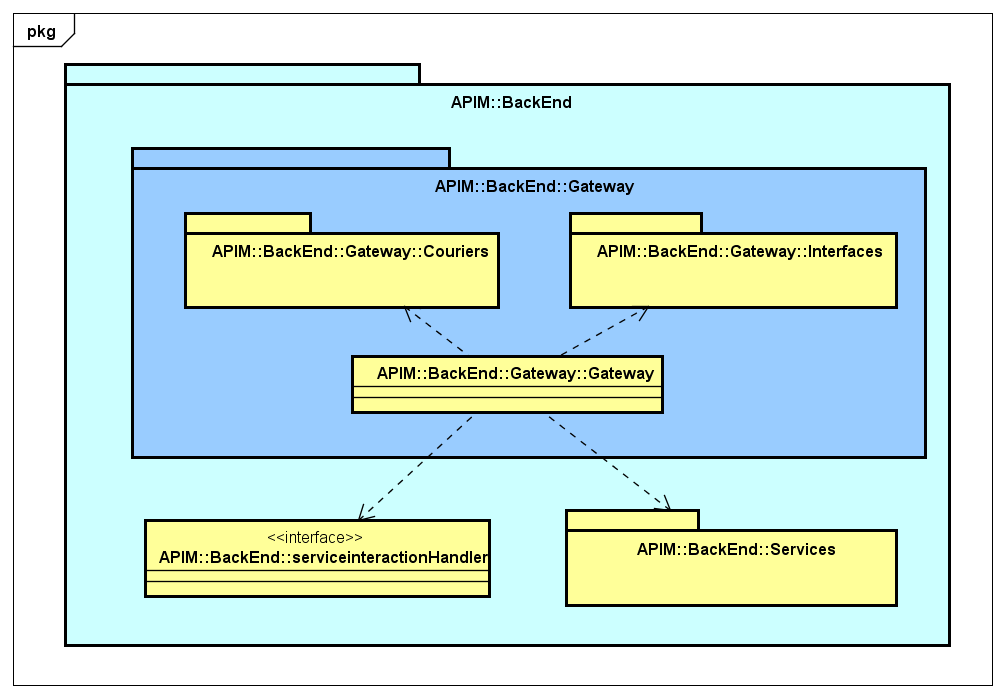
\includegraphics
	[width=0.7\linewidth]
	{UML/DiagrammiPackage/gateway.png}
	\caption{Package APIM::BackEnd::Gateway}
\end{figure}

\begin{itemize}
	\item \textbf{Padre}: BackEnd;
	
	\item \textbf{Descrizione}: package contenente la componente principale del lato back-end. Pur essendo integrato nella sistema, è un modulo che svolge funzioni separate alla piattaforma vera e propria: infatti, l'API Gateway si occupa di controllare e reindirizzare le chiamate effettuate dai clienti ai microservizi (prodotti) inseriti nel marketplace \progetto, verificandone la validità (credenziali, chiave) e monitorandone l'uso (SLA, utilizzi rimanenti).
	
	\item \textbf{Relazioni d'uso con altri componenti}: la classe \textit{Gateway} comunica con le classi contenute all'interno del package \textit{Services}. Inoltre, necessita delle interfacce contenute nel package \textit{Interfaces} e crea le sessioni \textit{couriers} Jolie, archiviandole nel package \textit{Couriers}.
	
	\item \textbf{Package contenuti}:
	\begin{itemize}
		\item \textbf{\textit{Couriers}}: package contenente l'archivio delle sessioni couriers dei microservizi Jolie. Le sessioni couriers vengono create dal gateway ed utilizzate da \textit{serviceinteractionhandler}. Inoltr, forniscono i dati necessari al funzionamento del package \textit{Interfaces}.\\
		Le sessioni couriers permettono l'overloading dei messaggi inviati nelle chiamate dei microservizi al gateway, così da allegare alla richiesta le informazioni per raggiungere il microservizio desiderato.
		
		\item \textbf{\textit{Interfaces}}: package contenente le interfacce necessarie al funzionamento dell'API Gateway. Si occupa dei dati riguardanti le chiamate ai microservizi, in particolar modo, il tipo di operazione richiesta e le informazioni riguardanti l'interfaccia del microservizio target.
	\end{itemize}
	\item \textbf{Classi contenute}:
		\begin{itemize}
			\item \textbf{\textit{Gateway}}: classe che rappresenta la struttura dell'API Gateway della piattaforma \progetto.
		\end{itemize}
\end{itemize}

\subsubsection{Services}
Tale package contiene tutti i servizi appartenenti al lato back-end della piattaforma, eccezion fatta per il gateway già descritto nella sezione soprastante. \textit{Services} contiene tutte le classi di comunicazione con i database che permetteranno il corretto funzionamento dell'applicazione.

\begin{figure}[H]
	\centering
	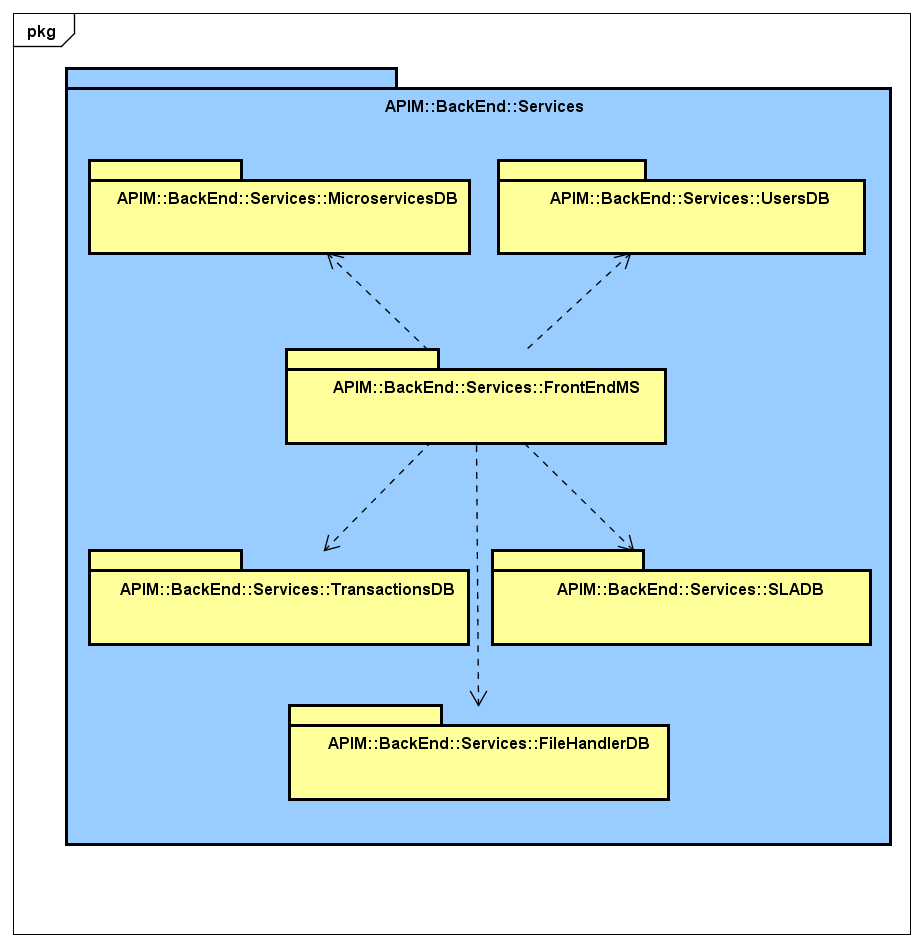
\includegraphics
	[width=0.7\linewidth]
	{UML/DiagrammiPackage/services.png}
	\caption{Package APIM::BackEnd::Services}
\end{figure}

\begin{itemize}
	\item \textbf{Padre}: BackEnd;
	
	\item \textbf{Descrizione}: package che contiene tutti i package relativi ai microservizi del back-end dell'applicazione;
	
	\item \textbf{Relazioni d'uso con altri componenti}: questo package si relaziona con l'API Gateway;
	
	\item \textbf{Package contenuti}:
	\begin{itemize}
		\item \textbf{\textit{UsersDB}}: package contenente le classi che permettono la comunicazione con il database relativo agli utenti del sistema;
		
		\item \textbf{\textit{MicroservicesDB}}: package contenente le classi che permettono la comunicazione con il database relativo ai microservizi registrati sulla piattaforma;
		
		\item \textbf{\textit{TransactionsDB}}: package contenente le classi che permettono la comunicazione con il database relativo alle transazioni degli utenti del sistema;
		
		\item \textbf{\textit{SLADB}}: package contenente le classi che permettono la comunicazione con il database relativo alle informazioni di SLA dei microservizi utilizzati tramite l'API Gateway della piattaforma \progetto;
		
		\item \textbf{\textit{FileHandlerDB}}: package contenente le classi che permettono la gestione dei file;
		
		\item \textbf{\textit{FrontEndMS}}: package contenente le classi che si occupano delle operazioni più complesse, quali l'accesso a più di un database.
	\end{itemize}
\end{itemize}

\paragraph{UsersDB}

\begin{figure}[H]
	\centering
	\includegraphics
	[width=0.7\linewidth]
	{UML/DiagrammiPackage/Users_db.png}
	\caption{Package APIM::BackEnd::Services::UsersDB}
\end{figure}

\begin{itemize}
	\item \textbf{Padre}: Services;
	
	\item \textbf{Descrizione}: package che contiene le classi di comunicazione con il database dell'applicazione relativo alle informazioni (anagrafiche e personali) degli utenti (admin, clienti, sviluppatori) del sistema;
	
	\item \textbf{Relazioni d'uso con altri componenti}: questo package si relaziona con il sub-package \textit{FrontEndMS} del package padre, fornendogli i dati che esso richiede riguardo alle operazioni con il database delle informazioni degli utenti;
	
	\item \textbf{Classi contenute}:
		\begin{itemize}
			\item \textbf{\textit{Users\_dbInterface}}: interfaccia che raccoglie tutte le \textit{operation} riguardanti il database degli utenti;
			
			\item \textbf{\textit{Users\_db}}: classe che implementa l'interfaccia \textit{Users\_dbInterface}.
		\end{itemize}
\end{itemize}

\paragraph{MicroservicesDB}

\begin{figure}[H]
	\centering
	\includegraphics
	[width=0.7\linewidth]
	{UML/DiagrammiPackage/MicroservicesDB.png}
	\caption{Package APIM::BackEnd::Services::MicroservicesDB}
\end{figure}

\begin{itemize}
	\item \textbf{Padre}: Services;
	
	\item \textbf{Descrizione}: package che contiene le classi di comunicazione con il database dell'applicazione relativo ai microservizi registrati nella piattaforma;
	
	\item \textbf{Relazioni d'uso con altri componenti}: questo package si relaziona con il package \textit{FrontendMS}, fornendogli i dati che esso richiede riguardo alle operazioni con il database delle informazioni dei microservizi.\\
	Inoltre, comunica con il Gateway per permettere l'identificazione e l'utilizzo dei microservizi, e garantire correttezza, efficienza e validità delle chiamate;
	
	\item \textbf{Classi contenute}:
	\begin{itemize}
		\item \textbf{\textit{Microservices\_dbInterface}}: interfaccia che raccoglie tutte le \textit{operation} riguardanti il database dei microservizi;
		
		\item \textbf{\textit{Microservices\_db}}: classe che implementa le interfacce \textit{Microservices\_dbInterface} e \textit{serviceInteractionHandler}.
	\end{itemize}
\end{itemize}

\paragraph{TransactionsDB}

\begin{figure}[H]
	\centering
	\includegraphics
	[width=0.7\linewidth]
	{UML/DiagrammiPackage/Transactions_db.png}
	\caption{Package APIM::BackEnd::Services::TransactionsDB}
\end{figure}

\begin{itemize}
	\item \textbf{Padre}: Services;
	
	\item \textbf{Descrizione}: package che contiene le classi di comunicazione con il database dell'applicazione che si occupa di immagazzinare i dati sulle transazioni;
	
	\item \textbf{Relazioni d'uso con altri componenti}: questo package si relaziona con il package \textit{FrontendMS}, fornendogli i dati che esso richiede riguardo alle operazioni con il database delle informazioni delle transazioni.\\
	Comunica inoltre con il Gateway per verificare la validità delle API Key e/o aggiornare i dati relativi (usi residui della chiave) alle chiamate ai microservizi effettuate;
	
	\item \textbf{Classi contenute}:
	\begin{itemize}
		\item \textbf{\textit{Transactions\_dbInterface}}: interfaccia che raccoglie tutte le \textit{operation} riguardanti il database delle transazioni;
		
		\item \textbf{\textit{Transactions\_db}}: classe che implementa l'interfaccia \textit{Transactions\_dbInterface}.
	\end{itemize}
\end{itemize}

\paragraph{SLADB}

\begin{figure}[H]
	\centering
	\includegraphics
	[width=0.7\linewidth]
	{UML/DiagrammiPackage/SLA_db.png}
	\caption{Package APIM::BackEnd::Services::SLADB}
\end{figure}

\begin{itemize}
	\item \textbf{Padre}: Services;
	
	\item \textbf{Descrizione}: package che contiene le classi di comunicazione con il database che si occupa di immagazzinare e trattare i dati relativi al Service Level Agreement (SLA);
	
	\item \textbf{Relazioni d'uso con altri componenti}: questo package si relaziona con il package \textit{FrontendMS}, fornendogli i dati che esso richiede riguardo alle operazioni con il database delle informazioni della SLA.\\
	Inoltre, comunica con il Gateway per aggiornare i dati delle performance di risposta di ogni microservizio utilizzato;
	
	\item \textbf{Classi contenute}:
	\begin{itemize}
		\item \textbf{\textit{SLA\_dbInterface}}: interfaccia che raccoglie tutte le \textit{operation} riguardanti il database delle informazioni di SLA;
		
		\item \textbf{\textit{SLA\_db}}: classe che implementa l'interfaccia \textit{SLA\_dbInterface}.
	\end{itemize}
\end{itemize}

\paragraph{FileHandlerDB}

\begin{figure}[H]
	\centering
	\includegraphics
	[width=0.7\linewidth]
	{UML/DiagrammiPackage/FileHandlerDB.png}
	\caption{Package APIM::BackEnd::Services::FileHandlerDB}
\end{figure}

\begin{itemize}
	\item \textbf{Padre}: Services;
	
	\item \textbf{Descrizione}: package che si occupa della gestione dei file, e presenta le classi di comunicazione con il database per tale finalità;
	
	\item \textbf{Relazioni d'uso con altri componenti}: questo package si relaziona con il package \textit{FrontendMS}, fornendogli i dati che esso richiede riguardo alle operazioni con il database delle informazioni dei file.\\
	Inoltre, comunica con il Gateway per recuperare i file legati alle interfacce dei microservizi;
	
	\item \textbf{Classi contenute}:
	\begin{itemize}
		\item \textbf{\textit{FileHandlerInterface}}: interfaccia che raccoglie tutte le \textit{operation} riguardanti la gestione dei file;
		
		\item \textbf{\textit{FileHandler}}: classe che implementa l'interfaccia \textit{FileHandlerInterface}.
	\end{itemize}
\end{itemize}

\paragraph{FrontendMS}

\begin{figure}[H]
	\centering
	\includegraphics
	[width=0.7\linewidth]
	{UML/DiagrammiPackage/FrontEndMS.png}
	\caption{Package APIM::BackEnd::Services::FrontEndMS}
\end{figure}

\begin{itemize}
	\item \textbf{Padre}: Services;
	
	\item \textbf{Descrizione}: package che si occupa delle operazioni più complesse, che accedono a più database e devono rielaborarne i dati. La maggior parte delle funzionalità garantite dal front-end passano per questo servizio, in quanto occorre raccogliere dati da più database e/o raffinare le informazioni grezze dei \textit{services};
	
	\item \textbf{Relazioni d'uso con altri componenti}: questo package si relaziona con tutti gli altri package e relativi servizi del package padre, quali \textit{UsersDB}, \textit{MicroservicesDB}, \textit{TransactionsDB}, \textit{SLADB} e \textit{FileHandlerDB};
	
	\item \textbf{Classi contenute}:
	\begin{itemize}
		\item \textbf{\textit{FrontEndInterface}}: interfaccia che raccoglie tutte le \textit{operation} più complesse, come ad esempio la gestione della visualizzazione della home del marketplace;
		
		\item \textbf{\textit{FrontEndMS}}: classe che implementa l'interfaccia \textit{FrontEndInterface}.
	\end{itemize}
\end{itemize}

\newpage
\section{Diagrammi di sequenza}

\subsection{Front-End}
I seguenti diagrammi di sequenza prendono in considerazione le principali operazioni del front-end e vanno ad illustrarne le interazioni tra le classi.

\subsubsection{Registrazione utente}

\begin{figure}[H]
	\centering
	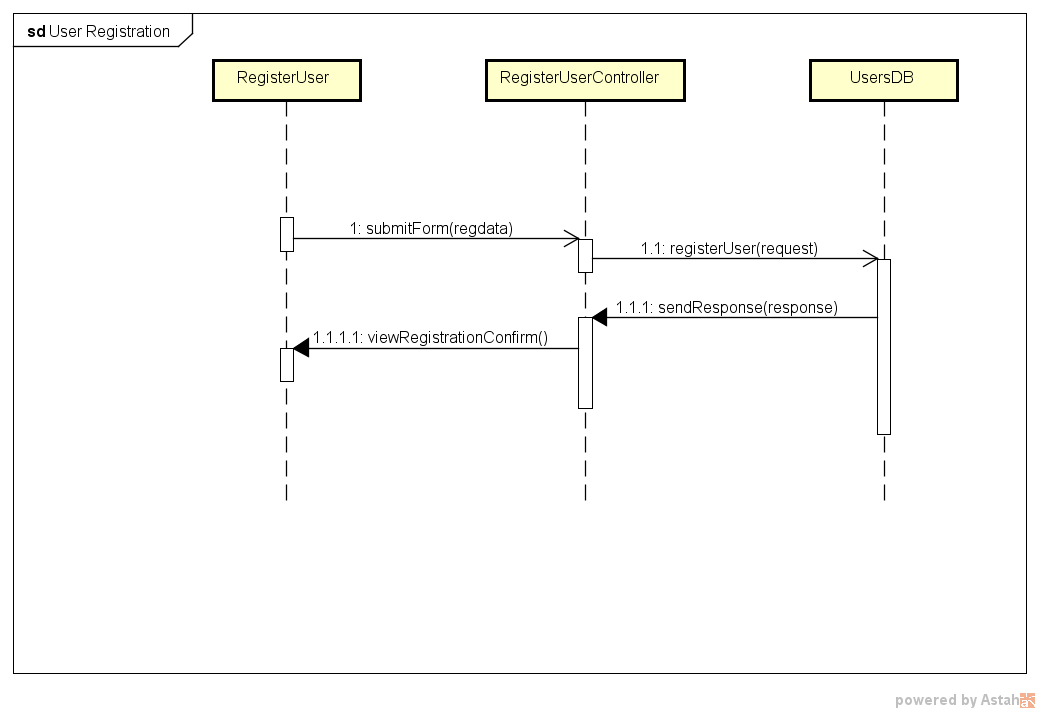
\includegraphics
	[width=0.7\linewidth]
	{UML/DiagrammiSequenza/registrazione_utente.png}
	\caption{Diagramma di sequenza: Registrazione utente}
\end{figure}

\begin{itemize}
	\item \textbf{Pre-condizioni}: l'utente si trova nella schermata di registrazione utente;
	\item \textbf{Post-condizioni}: l'utente ha compilato il form per la registrazione ed ora possiede le credenziali per l'autenticazione alla piattaforma API Market;
	\item \textbf{Descrizione}: l'utente compila il form per la registrazione di un account, provvedendo ad inserire tutte le informazioni obbligatorie richieste. Confermando la registrazione, i services di API Market provvedono ad inserire nel database il nuovo utente. A registrazione avvenuta, l'utente riceve un messaggio di successo e viene reindirizzato alla pagina di login.
\end{itemize}


\subsubsection{Autenticazione}

\begin{figure}[H]
	\centering
	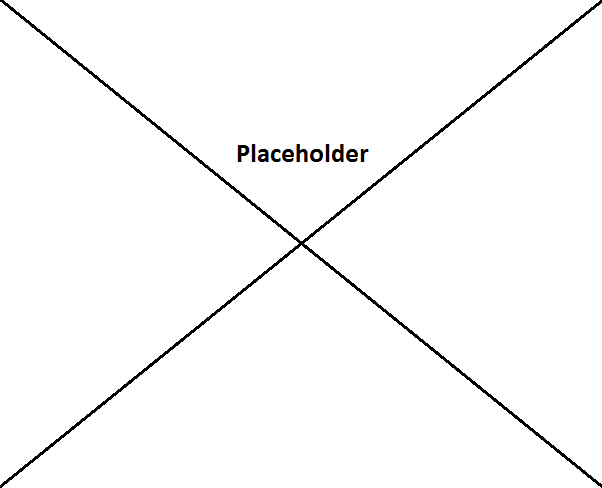
\includegraphics
	[width=0.7\linewidth]
	{UML/DiagrammiSequenza/login.png}
	\caption{Diagramma di sequenza: Autenticazione}
\end{figure}

\begin{itemize}
	\item \textbf{Pre-condizioni}: l'utente si trova nella schermata di autenticazione;
	\item \textbf{Post-condizioni}: l'utente ha compilato il form per il login ed ora risulta un utente autenticato al sistema API Market;
	\item \textbf{Descrizione}: l'utente compila il form per l'autenticazione, provvedendo ad inserire la propria email e password con le quali si era registrato. Confermando l'autenticazione, la piattaforma API Market provvede a creare una sessione per l'utente autenticato, il quale, nel caso di autenticazione avvenuta con successo, viene reindirizzato alla home dell'applicazione.
\end{itemize}
\clearpage

\subsubsection{Recupero password}

\begin{figure}[H]
	\centering
	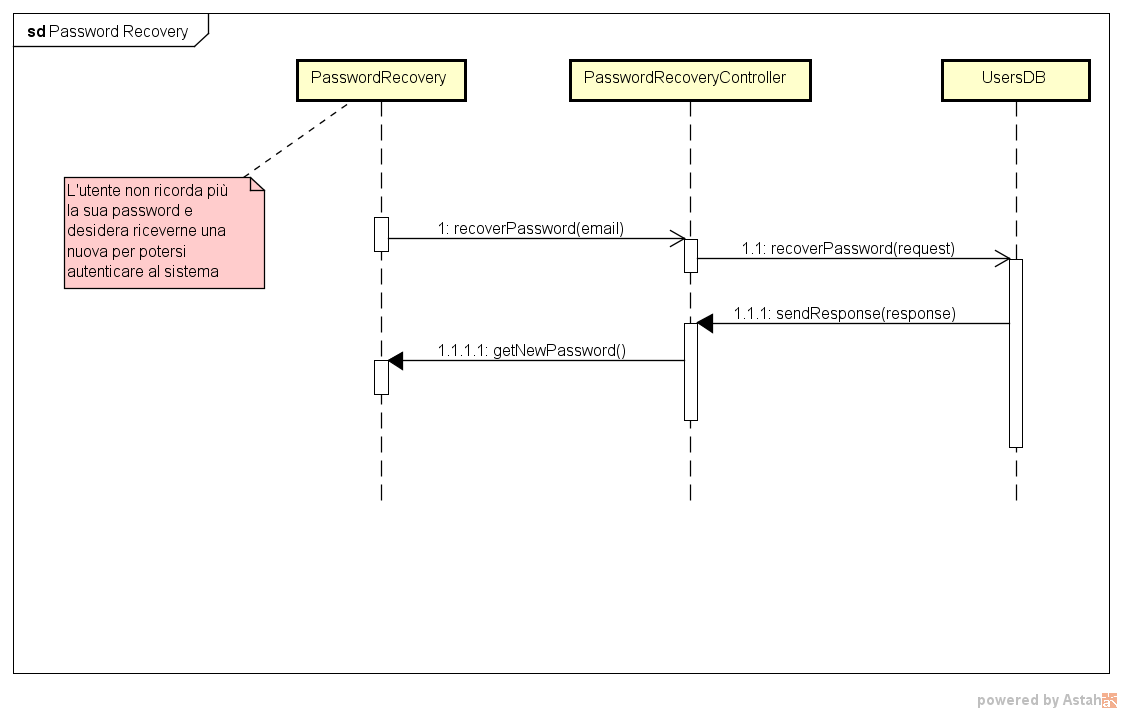
\includegraphics
	[width=0.7\linewidth]
	{UML/DiagrammiSequenza/recupero_password.png}
	\caption{Diagramma di sequenza: Recupero password}
\end{figure}

\begin{itemize}
	\item \textbf{Pre-condizioni}: l'utente si trova nella schermata di recupero password;
	\item \textbf{Post-condizioni}: l'utente ha compilato il form per il recupero della propria password tramite email ed ora può ri-effettuare l'autenticazione alla piattaforma API Market;
	\item \textbf{Descrizione}: l'utente compila il form per il recupero della password relativa al proprio account, inserendo l'email dove il sistema inoltrerà la nuova password generata. Confermando l'operazione, i services di API Market provvedono ad aggiornare il campo password nel database degli utenti. A recupero avvenuto, l'utente riceve un messaggio di successo e viene reindirizzato alla pagina di login.
\end{itemize}
\clearpage

\subsubsection{Ricerca API}

\begin{figure}[H]
	\centering
	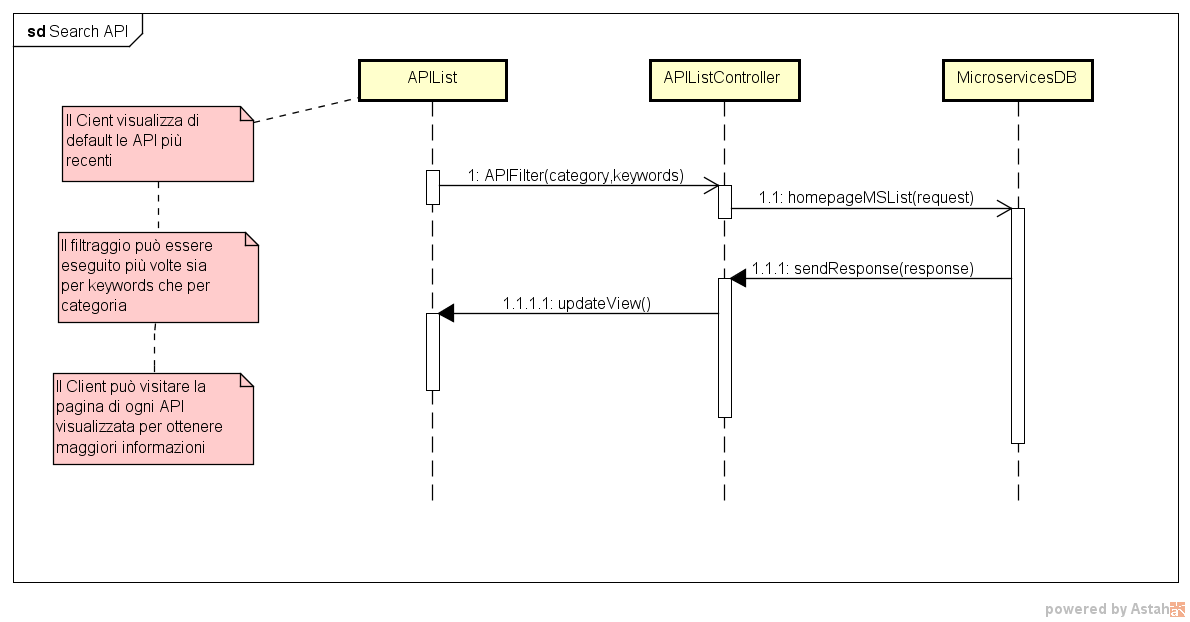
\includegraphics
	[width=0.7\linewidth]
	{UML/DiagrammiSequenza/ricercaAPI.png}
	\caption{Diagramma di sequenza: Ricerca API}
\end{figure}

\begin{itemize}
	\item \textbf{Pre-condizioni}: l'utente si trova nella homepage dell'applicazione;
	\item \textbf{Post-condizioni}: l'utente ha visualizzato le API secondo la categoria e le keywords inserite;
	\item \textbf{Descrizione}: di default, la homepage di API Market mostra le API registrate più recentemente. L'utente può immettere delle keywords nell'apposito riquadro per alterare i risultati, e scegliere di restringere la ricerca ad una singola categoria. I risultati visualizzati cambiano dinamicamente non appena l'applicazione web riceve risposta dai servizi che la collegano ai database.
\end{itemize}
\clearpage

\subsubsection{Acquisto API}

\begin{figure}[H]
	\centering
	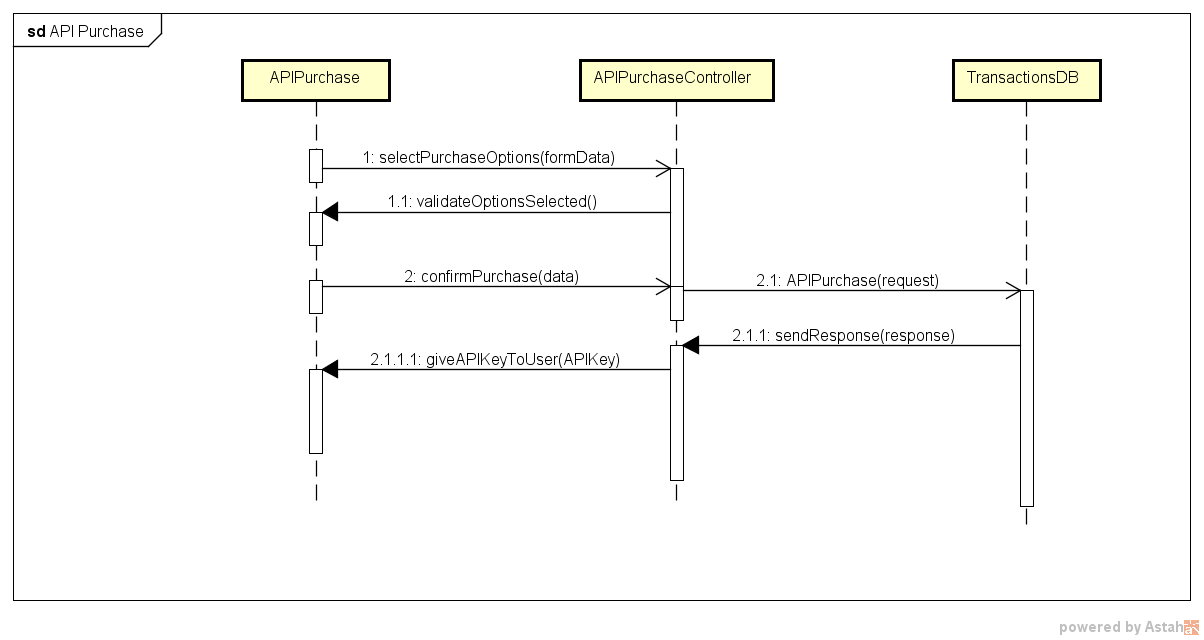
\includegraphics
	[width=0.7\linewidth]
	{UML/DiagrammiSequenza/acquistoAPI.png}
	\caption{Diagramma di sequenza: Acquisto API}
\end{figure}

\begin{itemize}
	\item \textbf{Pre-condizioni}: il cliente si trova nella schermata di acquisto di una specifica API;
	\item \textbf{Post-condizioni}: il cliente ha ricevuto l'API Key per l'API acquistata, secondo le modalità da lui scelte, e gli sono stati sottratti i corrispondenti crediti;
	\item \textbf{Descrizione}: il cliente compila il form per l'acquisto dell'API desiderata, visualizzando il preventivo di crediti spesi in base ai parametri scelti. Confermando l'acquisto (che può essere anche un rinnovo), i services di API Market provvedono a generare una apikey ed a scalare i crediti dall'account utente. L'utente potrà visualizzare l'API Key ed un messaggio di ringraziamento.
\end{itemize}
\clearpage

\subsubsection{Inserimento API}

\begin{figure}[H]
	\centering
	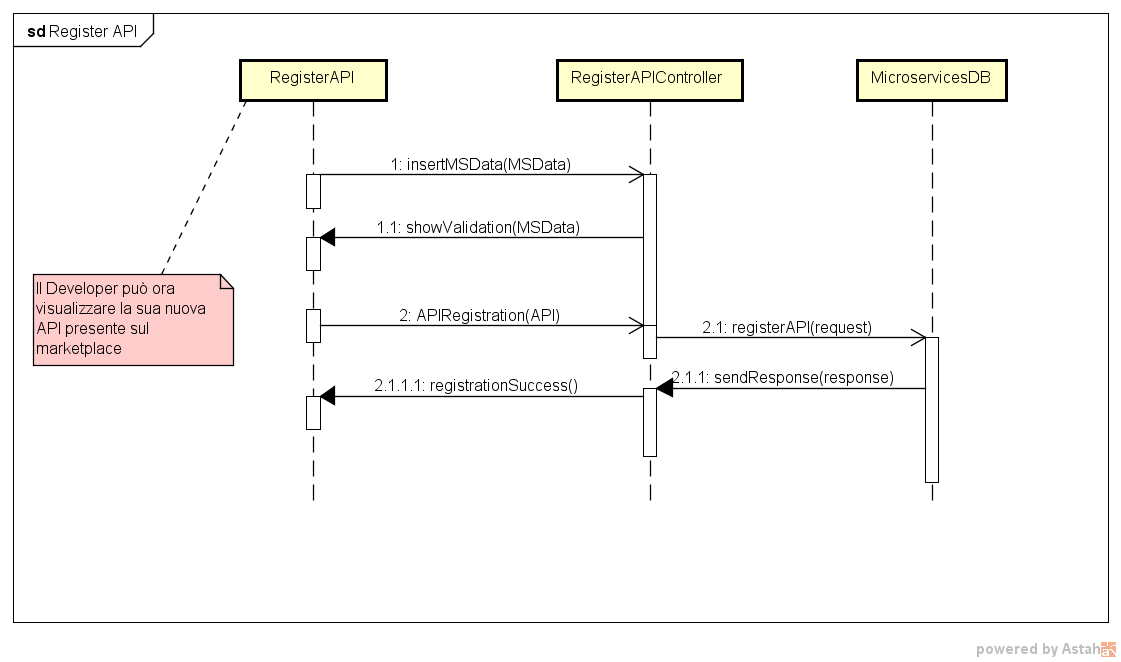
\includegraphics
	[width=0.7\linewidth]
	{UML/DiagrammiSequenza/registrazioneAPI.png}
	\caption{Diagramma di sequenza: Inserimento API}
\end{figure}

\begin{itemize}
	\item \textbf{Pre-condizioni}: lo sviluppatore si trova nella schermata di registrazione di una nuova API;
	\item \textbf{Post-condizioni}: lo sviluppatore ha registrato la sua nuova API ed essa è ora disponibile in API Market;
	\item \textbf{Descrizione}: lo sviluppatore compila il form per la registrazione di una nuova API, provvedendo anche a caricare sul server di API Market i file del logo e della documentazione PDF. Confermando la registrazione, i services di API Market provvedono ad inserire nel database la nuova API e renderla accessibile attraverso il Gateway. A registrazione avvenuta, lo sviluppatore riceve un messaggio di successo.
\end{itemize}
\clearpage

\subsubsection{Ricarica saldo conto virtuale}

\begin{figure}[H]
	\centering
	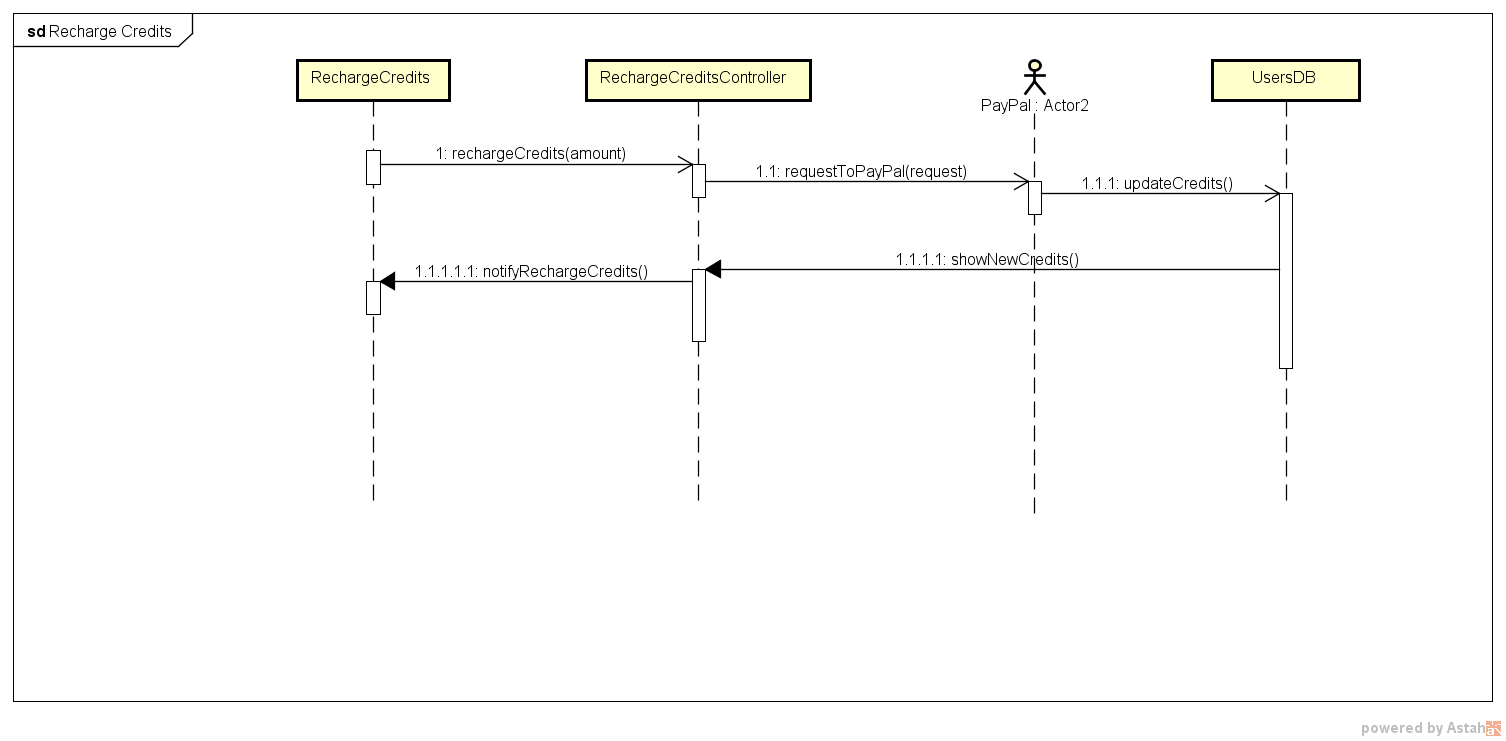
\includegraphics
	[width=0.7\linewidth]
	{UML/DiagrammiSequenza/ricaricaCrediti.png}
	\caption{Diagramma di sequenza: Ricarica saldo conto virtuale}
\end{figure}

\begin{itemize}
	\item \textbf{Pre-condizioni}: il cliente si trova nella schermata di ricarica del proprio conto virtuale;
	\item \textbf{Post-condizioni}: il cliente ha effettuato la ricarica dei propri crediti;
	\item \textbf{Descrizione}: il cliente stabilisce l'ammontare dei crediti da ricaricare nel proprio conto virtuale. A decisione avvenuta, verrà reindirizzato alla procedura di acquisto di PayPal, che lo guiderà nell'acquisto. Portata a termine la transazione, PayPal avvertirà i services di API Market che si occuperanno di incrementare i crediti del conto virtuale del cliente.
\end{itemize}


%\subsection{Back-End}
%I seguenti diagrammi di sequenza prendono in considerazione le principali operazioni del back-end e vanno ad illustrarne le interazioni tra le classi.

\newpage
\renewcommand*{\arraystretch}{1.6}

\section{Tracciamento componenti}
\textbf{N.B.}: il tracciamento Componenti-Requisiti del package \textit{APIGateway} è stato omesso, in quanto esso si occupa della chiamate ai microservizi, che sono estranei alla nostra responsabilità.

\subsection{Tracciamento componenti-requisiti}
		\begin{longtable}{ p{12cm} | p{4cm} }
			\hline \rowcolor{Gray}
			\textbf{Nome Componente} & \textbf{Codice Requisito} \\
			\hline
			APIM::FrontEnd
			& RFO1 \\
			& RFO1.1 \\
			& RFO1.2 \\
			& RFO1.3 \\
			& RFO1.4 \\
			& RFO1.5 \\
			& RFO1.6 \\
			& RFO1.7 \\
			& RFO1.8 \\
			& RFO1.9 \\
			& RFO1.10 \\
			& RFO2 \\
			& RFO2.1 \\
			& RFO2.1.1 \\
			& RFO2.1.2 \\
			& RFO2.1.3 \\
			& RFO2.1.4 \\
			& RFD3 \\
			& RFD3.1 \\
			& RFD3.2 \\
			& RFD3.3 \\
			& RFD3.4 \\
			& RFO4 \\
			& RFO4.1 \\
			& RFO4.2 \\
			& RFO4.3 \\
			& RFO4.3.1 \\
			& RFO4.3.2 \\
			& RFO4.3.3 \\
			& RFO4.3.4 \\
			& RFO4.3.5 \\
			& RFO5 \\
			& RFO5.1 \\
			& RFO5.2 \\
			& RFO5.3 \\
			& RFO5.4 \\
			& RFO5.5 \\
			& RFO5.5.1 \\
			& RFO5.5.2 \\
			& RFO5.6 \\
			& RFO5.6.1 \\
			& RFO5.6.2 \\
			& RFO5.7 \\
			& RFD5.7.1 \\
			& RFO5.7.2 \\
			& RFO5.8 \\
			& RFO5.9 \\
			& RFO5.10 \\
			& RFO5.11 \\
			& RFO5.12 \\
			& RFO5.13 \\
			& RFO6 \\
			& RFO6.1 \\
			& RFO6.2 \\
			& RFO6.2.1 \\
			& RFO6.2.2 \\
			& RFO6.2.3 \\
			& RFO6.2.4 \\
			& RFO6.2.5 \\
			& RFD6.2.6 \\
			& RFD6.2.7 \\
			& RFO7 \\
			& RFO7.1 \\
			& RFO7.1.1 \\
			& RFO7.1.2 \\
			& RFO7.1.3 \\
			& RFO7.2 \\
			& RFO7.3 \\
			& RFO7.4 \\
			& RFO7.5 \\
			& RFD7.5.1 \\
			& RFO7.5.2 \\
			& RFO7.5.3 \\
			& RFO7.6 \\
			& RFO8 \\
			& RFO8.1 \\
			& RFO8.2 \\
			& RFO8.2.1 \\
			& RFO8.2.2 \\
			& RFO8.2.3 \\
			& RFO8.2.4 \\
			& RFO8.2.4.1 \\
			& RFO8.2.4.2 \\
			& RFD8.2.4.3 \\
			& RFO8.2.4.4 \\
			& RFO8.2.4.5 \\
			& RFO8.2.4.6 \\
			& RFO8.2.4.7 \\
			& RFO8.2.4.8 \\
			& RFO8.2.4.9 \\
			& RFO8.2.4.10 \\
			& RFO8.2.4.11 \\
			& RFO8.2.5 \\
			& RFO8.2.6 \\
			& RFO8.2.7 \\
			& RFO8.2.8 \\
			& RFO8.2.9 \\
			& RFO8.2.9.1 \\
			& RFO8.2.9.2 \\
			& RFO9 \\
			& RFO9.1 \\
			& RFO9.2 \\
			& RFO9.3 \\
			& RFO9.4 \\
			& RFO9.5 \\
			& RFD9.6 \\
			& RFD9.7 \\
			& RFO9.8 \\
			& RFO9.8.1 \\
			& RFO9.8.2 \\
			& RFO9.8.3 \\
			& RFO9.9 \\
			& RFD9.10 \\
			& RFD9.11 \\
			& RFO9.12 \\
			& RFD9.13 \\
			& RFO10 \\
			& RFO10.1 \\
			& RFO10.1.1 \\
			& RFO10.1.1.1 \\
			& RFO10.1.1.2 \\
			& RFO10.1.1.3 \\
			& RFO10.1.1.4 \\
			& RFO10.1.1.5 \\
			& RFO10.1.1.6 \\
			& RFO10.1.2 \\
			& RFO10.1.2.1 \\
			& RFO10.1.2.2 \\
			& RFO10.1.2.3 \\
			& RFO10.1.2.4 \\
			& RFO10.1.2.5 \\
			& RFD10.1.2.6 \\
			& RFO10.1.2.7 \\
			& RFO10.1.2.8 \\
			& RFD10.1.2.8 \\
			& RFO10.2 \\
			& RFO11 \\
			& RFO12 \\
			& RFO12.1 \\
			& RFO12.1.1 \\
			& RFO12.1.1.1 \\
			& RFO12.1.1.1.1 \\
			& RFO12.1.1.1.2 \\
			& RFD12.1.1.1.3 \\
			& RFD12.1.1.1.4 \\
			& RFO12.1.1.1.5 \\
			& RFO12.1.1.1.5.1 \\
			& RFF12.1.1.1.5.2 \\
			& RFD12.1.1.1.6 \\
			& RFO12.1.1.2 \\
			& RFO12.1.1.2.1 \\
			& RFO12.1.1.2.2 \\
			& RFD12.1.1.3 \\
			& RFO12.1.1.3.1 \\
			& RFD12.1.1.3.2 \\
			& RFO12.1.1.3.3 \\
			& RFO12.2 \\
			& RFO12.2.1 \\
			& RFO12.2.1.1 \\
			& RFO12.2.1.1.1 \\
			& RFO12.2.1.1.2 \\
			& RFO12.2.1.2 \\
			& RFO12.2.1.2.1 \\
			& RFO12.2.1.2.2 \\
			& RFO12.2.1.3 \\
			& RFO12.2.1.4 \\
			& RFO12.2.1.5 \\
			& RFO12.2.1.5.1 \\
			& RFO12.2.1.5.2 \\
			\hline
			APIM::BackEnd
			& RFO1 \\
			& RFO1.1 \\
			& RFO1.2 \\
			& RFO1.3 \\
			& RFO1.4 \\
			& RFO1.5 \\
			& RFO1.6 \\
			& RFO1.7 \\
			& RFO1.8 \\
			& RFO1.9 \\
			& RFO1.10 \\
			& RFO4.3.1 \\
			& RFO4.3.2 \\
			& RFO4.3.3 \\
			& RFD4.3.4 \\
			& RFO4.3.5 \\
			& RFO5 \\
			& RFO5.1 \\
			& RFO5.2 \\
			& RFO5.3 \\
			& RFO5.4 \\
			& RFO5.5 \\
			& RFO5.5.1 \\
			& RFO5.5.2 \\
			& RFO5.6 \\
			& RFO5.6.1 \\
			& RFO5.6.2 \\
			& RFO5.7 \\
			& RFD5.7.1 \\
			& RFO5.7.2 \\
			& RFO5.8 \\
			& RFO5.9 \\
			& RFO5.10 \\
			& RFO5.11 \\
			& RFO5.12 \\
			& RFO5.13 \\
			& RFO6 \\
			& RFO6.1 \\
			& RFO6.2 \\
			& RFO6.2.1 \\
			& RFO6.2.2 \\
			& RFO6.2.3 \\
			& RFO6.2.4 \\
			& RFO6.2.5 \\
			& RFD6.2.6 \\
			& RFD6.2.7 \\
			& RFO7 \\
			& RFO7.1 \\
			& RFO7.1.1 \\
			& RFO7.1.2 \\
			& RFO7.1.3 \\
			& RFO7.2 \\
			& RFO7.3 \\
			& RFO7.4 \\
			& RFO7.5 \\
			& RFD7.5.1 \\
			& RFO7.5.2 \\
			& RFO7.5.3 \\
			& RFO7.6 \\
			& RFO8 \\
			& RFO8.1 \\
			& RFO8.2 \\
			& RFO8.2.1 \\
			& RFO8.2.2 \\
			& RFO8.2.3 \\
			& RFO8.2.4 \\
			& RFO8.2.4.1 \\
			& RFO8.2.4.2 \\
			& RFD8.2.4.3 \\
			& RFO8.2.4.4 \\
			& RFO8.2.4.5 \\
			& RFO8.2.4.6 \\
			& RFO8.2.4.7 \\
			& RFO8.2.4.8 \\
			& RFO8.2.4.9 \\
			& RFO8.2.4.10 \\
			& RFO8.2.4.11 \\
			& RFO8.2.5 \\
			& RFO8.2.6 \\
			& RFO8.2.7 \\
			& RFO8.2.8 \\
			& RFO8.2.9 \\
			& RFO8.2.9.1 \\
			& RFO8.2.9.2 \\
			& RFO9 \\
			& RFO9.1 \\
			& RFO9.2 \\
			& RFD9.3 \\
			& RFO9.4 \\
			& RFO9.5 \\
			& RFD9.6 \\
			& RFD9.7 \\
			& RFO9.8 \\
			& RFO9.8.1 \\
			& RFO9.8.2 \\
			& RFO9.8.3 \\
			& RFO9.9 \\
			& RFD9.10 \\
			& RFD9.11 \\
			& RFO9.12 \\
			& RFD9.13 \\
			& RFO10 \\
			& RFO10.1 \\
			& RFO10.1.1 \\
			& RFO10.1.1.1 \\
			& RFO10.1.1.2 \\
			& RFO10.1.1.3 \\
			& RFO10.1.1.4 \\
			& RFO10.1.1.5 \\
			& RFO10.1.1.6 \\
			& RFO10.1.2 \\
			& RFO10.1.2.1 \\
			& RFO10.1.2.2 \\
			& RFO10.1.2.3 \\
			& RFO10.1.2.4 \\
			& RFO10.1.2.5 \\
			& RFD10.1.2.6 \\
			& RFO10.1.2.7 \\
			& RFO10.1.2.8 \\
			& RFD10.1.2.8 \\
			& RFO10.2 \\
			& RFO10.2.1 \\
			& RFO10.2.2 \\
			& RFO10.2.2.1 \\
			& RFO10.2.2.2 \\
			& RFO10.3.3 \\
			& RFO10.3.3.1 \\
			& RFO10.3.3.2 \\
			& RFO10.3.3.3 \\
			& RFO10.3.3.4 \\
			& RF010.3 \\
			& RF010.3.1 \\
			& RF010.3.1.1 \\
			& RF010.3.1.2 \\
			& RF010.3.2 \\
			& RF010.3.2.1 \\
			& RF010.3.2.2 \\
			& RF010.3.2.3 \\
			& RF010.3.2.4 \\
			& RF010.3.2.5 \\
			& RFO11 \\							

			\hline
			APIM::FrontEnd::App::Index
			& RFO1 \\
			& RFO2 \\
			& RFO4 \\
			& RFO4.1 \\
			& RFO4.2 \\
			& RFO4.3 \\
			& RFO4.3.1 \\
			& RFO4.3.2 \\
			& RFO4.3.3 \\
			& RFO4.3.4 \\
			& RFO4.3.5 \\
			& RFO11 \\
			\hline
			APIM::FrontEnd::App::Views
			& RFO1 \\
			& RFO1.1 \\
			& RFO1.2 \\
			& RFO1.3 \\
			& RFO1.4 \\
			& RFO1.5 \\
			& RFO1.6 \\
			& RFO1.7 \\
			& RFO1.8 \\
			& RFO1.9 \\
			& RFO1.10 \\
			& RFO2 \\
			& RFO2.1 \\
			& RFO2.1.1 \\
			& RFO2.1.2 \\
			& RFO2.1.3 \\
			& RFO2.1.4 \\
			& RFD3 \\
			& RFD3.1 \\
			& RFD3.2 \\
			& RFD3.3 \\
			& RFD3.4 \\
			& RFO4 \\
			& RFO4.1 \\
			& RFO4.2 \\
			& RFO4.3 \\
			& RFO4.3.1 \\
			& RFO4.3.2 \\
			& RFO4.3.3 \\
			& RFO4.3.4 \\
			& RFO4.3.5 \\
			& RFO5 \\
			& RFO5.1 \\
			& RFO5.2 \\
			& RFO5.3 \\
			& RFO5.4 \\
			& RFO5.5 \\
			& RFO5.5.1 \\
			& RFO5.5.2 \\
			& RFO5.6 \\
			& RFO5.6.1 \\
			& RFO5.6.2 \\
			& RFO5.7 \\
			& RFD5.7.1 \\
			& RFO5.7.2 \\
			& RFO5.8 \\
			& RFO5.9 \\
			& RFO5.10 \\
			& RFO5.11 \\
			& RFO5.12 \\
			& RFO5.13 \\
			& RFO6 \\
			& RFO6.1 \\
			& RFO6.2 \\
			& RFO6.2.1 \\
			& RFO6.2.2 \\
			& RFO6.2.3 \\
			& RFO6.2.4 \\
			& RFO6.2.5 \\
			& RFD6.2.6 \\
			& RFD6.2.7 \\
			& RFO7 \\
			& RFO7.1 \\
			& RFO7.1.1 \\
			& RFO7.1.2 \\
			& RFO7.1.3 \\
			& RFO7.2 \\
			& RFO7.3 \\
			& RFO7.4 \\
			& RFO7.5 \\
			& RFD7.5.1 \\
			& RFO7.5.2 \\
			& RFO7.5.3 \\
			& RFO7.6 \\
			& RFO8 \\
			& RFO8.1 \\
			& RFO8.2 \\
			& RFO8.2.1 \\
			& RFO8.2.2 \\
			& RFO8.2.3 \\
			& RFO8.2.4 \\
			& RFO8.2.4.1 \\
			& RFO8.2.4.2 \\
			& RFD8.2.4.3 \\
			& RFO8.2.4.4 \\
			& RFO8.2.4.5 \\
			& RFO8.2.4.6 \\
			& RFO8.2.4.7 \\
			& RFO8.2.4.8 \\
			& RFO8.2.4.9 \\
			& RFO8.2.4.10 \\
			& RFO8.2.4.11 \\
			& RFO8.2.5 \\
			& RFO8.2.6 \\
			& RFO8.2.7 \\
			& RFO8.2.8 \\
			& RFO8.2.9 \\
			& RFO8.2.9.1 \\
			& RFO8.2.9.2 \\
			& RFO9 \\
			& RFO9.1 \\
			& RFO9.2 \\
			& RFO9.3 \\
			& RFO9.4 \\
			& RFO9.5 \\
			& RFD9.6 \\
			& RFD9.7 \\
			& RFO9.8 \\
			& RFO9.8.1 \\
			& RFO9.8.2 \\
			& RFO9.8.3 \\
			& RFO9.9 \\
			& RFD9.10 \\
			& RFD9.11 \\
			& RFO9.12 \\
			& RFD9.13 \\
			& RFO10 \\
			& RFO10.1 \\
			& RFO10.1.1 \\
			& RFO10.1.1.1 \\
			& RFO10.1.1.2 \\
			& RFO10.1.1.3 \\
			& RFO10.1.1.4 \\
			& RFO10.1.1.5 \\
			& RFO10.1.1.6 \\
			& RFO10.1.2 \\
			& RFO10.1.2.1 \\
			& RFO10.1.2.2 \\
			& RFO10.1.2.3 \\
			& RFO10.1.2.4 \\
			& RFO10.1.2.5 \\
			& RFD10.1.2.6 \\
			& RFO10.1.2.7 \\
			& RFO10.1.2.8 \\
			& RFD10.1.2.8 \\
			& RFO10.2 \\
			& RFO11 \\
			& RFO12 \\
			& RFO12.1 \\
			& RFO12.1.1 \\
			& RFO12.1.1.1 \\
			& RFO12.1.1.1.1 \\
			& RFO12.1.1.1.2 \\
			& RFD12.1.1.1.3 \\
			& RFD12.1.1.1.4 \\
			& RFO12.1.1.1.5 \\
			& RFO12.1.1.1.5.1 \\
			& RFF12.1.1.1.5.2 \\
			& RFD12.1.1.1.6 \\
			& RFO12.1.1.2 \\
			& RFO12.1.1.2.1 \\
			& RFO12.1.1.2.2 \\
			& RFD12.1.1.3 \\
			& RFO12.1.1.3.1 \\
			& RFD12.1.1.3.2 \\
			& RFO12.1.1.3.3 \\
			& RFO12.2 \\
			& RFO12.2.1 \\
			& RFO12.2.1.1 \\
			& RFO12.2.1.1.1 \\
			& RFO12.2.1.1.2 \\
			& RFO12.2.1.2 \\
			& RFO12.2.1.2.1 \\
			& RFO12.2.1.2.2 \\
			& RFO12.2.1.3 \\
			& RFO12.2.1.4 \\
			& RFO12.2.1.5 \\
			& RFO12.2.1.5.1 \\
			& RFO12.2.1.5.2 \\
			\hline
			APIM::FrontEnd::App::Models
			& RFO1 \\
			& RFO1.1 \\
			& RFO1.2 \\
			& RFO1.3 \\
			& RFO1.4 \\
			& RFO1.5 \\
			& RFO1.6 \\
			& RFO1.7 \\
			& RFO1.8 \\
			& RFO1.9 \\
			& RFO1.10 \\
			& RFO4.3.1 \\
			& RFO4.3.2 \\
			& RFO4.3.3 \\
			& RFO4.3.4 \\
			& RFO4.3.5 \\
			& RFO5 \\
			& RFO5.1 \\
			& RFO5.2 \\
			& RFO5.3 \\
			& RFO5.4 \\
			& RFO5.5 \\
			& RFO5.5.1 \\
			& RFO5.5.2 \\
			& RFO5.6 \\
			& RFO5.6.1 \\
			& RFO5.6.2 \\
			& RFO5.7 \\
			& RFD5.7.1 \\
			& RFO5.7.2 \\
			& RFO5.8 \\
			& RFO5.9 \\
			& RFO5.10 \\
			& RFO5.11 \\
			& RFO5.12 \\
			& RFO5.13 \\
			& RFO6 \\
			& RFO6.1 \\
			& RFO6.2 \\
			& RFO6.2.1 \\
			& RFO6.2.2 \\
			& RFO6.2.3 \\
			& RFO6.2.4 \\
			& RFO6.2.5 \\
			& RFD6.2.6 \\
			& RFD6.2.7 \\
			& RFO7 \\
			& RFO7.1 \\
			& RFO7.1.1 \\
			& RFO7.1.2 \\
			& RFO7.1.3 \\
			& RFO7.2 \\
			& RFO7.3 \\
			& RFO7.4 \\
			& RFO7.5 \\
			& RFD7.5.1 \\
			& RFO7.5.2 \\
			& RFO7.5.3 \\
			& RFO7.6 \\
			& RFO8 \\
			& RFO8.1 \\
			& RFO8.2 \\
			& RFO8.2.1 \\
			& RFO8.2.2 \\
			& RFO8.2.3 \\
			& RFO8.2.4 \\
			& RFO8.2.4.1 \\
			& RFO8.2.4.2 \\
			& RFD8.2.4.3 \\
			& RFO8.2.4.4 \\
			& RFO8.2.4.5 \\
			& RFO8.2.4.6 \\
			& RFO8.2.4.7 \\
			& RFO8.2.4.8 \\
			& RFO8.2.4.9 \\
			& RFO8.2.4.10 \\
			& RFO8.2.4.11 \\
			& RFO8.2.5 \\
			& RFO8.2.6 \\
			& RFO8.2.7 \\
			& RFO8.2.8 \\
			& RFO8.2.9 \\
			& RFO8.2.9.1 \\
			& RFO8.2.9.2 \\
			& RFO9 \\
			& RFO9.1 \\
			& RFO9.2 \\
			& RFD9.3 \\
			& RFO9.4 \\
			& RFO9.5 \\
			& RFD9.6 \\
			& RFD9.7 \\
			& RFO9.8 \\
			& RFO9.8.1 \\
			& RFO9.8.2 \\
			& RFO9.8.3 \\
			& RFO9.9 \\
			& RFD9.10 \\
			& RFD9.11 \\
			& RFO9.12 \\
			& RFD9.13 \\
			& RFO10 \\
			& RFO10.1 \\
			& RFO10.1.1 \\
			& RFO10.1.1.1 \\
			& RFO10.1.1.2 \\
			& RFO10.1.1.3 \\
			& RFO10.1.1.4 \\
			& RFO10.1.1.5 \\
			& RFO10.1.1.6 \\
			& RFO10.1.2 \\
			& RFO10.1.2.1 \\
			& RFO10.1.2.2 \\
			& RFO10.1.2.3 \\
			& RFO10.1.2.4 \\
			& RFO10.1.2.5 \\
			& RFD10.1.2.6 \\
			& RFO10.1.2.7 \\
			& RFO10.1.2.8 \\
			& RFD10.1.2.8 \\
			& RFO10.2 \\
			& RFO10.2.1 \\
			& RFO10.2.2 \\
			& RFO10.2.2.1 \\
			& RFO10.2.2.2 \\
			& RFO10.3.3 \\
			& RFO10.3.3.1 \\
			& RFO10.3.3.2 \\
			& RFO10.3.3.3 \\
			& RFO10.3.3.4 \\
			& RFO11 \\
			\hline
			APIM::FrontEnd::App::Controllers
			& RFO1 \\
			& RFO1.1 \\
			& RFO1.2 \\
			& RFO1.3 \\
			& RFO1.4 \\
			& RFO1.5 \\
			& RFO1.6 \\
			& RFO1.7 \\
			& RFO1.8 \\
			& RFO1.9 \\
			& RFO1.10 \\
			& RFO2 \\
			& RFO2.1 \\
			& RFO2.1.1 \\
			& RFO2.1.2 \\
			& RFO2.1.3 \\
			& RFO2.1.4 \\
			& RFD3 \\
			& RFD3.1 \\
			& RFD3.2 \\
			& RFD3.3 \\
			& RFD3.4 \\
			& RFO4 \\
			& RFO4.1 \\
			& RFO4.2 \\
			& RFO4.3 \\
			& RFO4.3.1 \\
			& RFO4.3.2 \\
			& RFO4.3.3 \\
			& RFO4.3.4 \\
			& RFO4.3.5 \\
			& RFO5 \\
			& RFO5.1 \\
			& RFO5.2 \\
			& RFO5.3 \\
			& RFO5.4 \\
			& RFO5.5 \\
			& RFO5.5.1 \\
			& RFO5.5.2 \\
			& RFO5.6 \\
			& RFO5.6.1 \\
			& RFO5.6.2 \\
			& RFO5.7 \\
			& RFD5.7.1 \\
			& RFO5.7.2 \\
			& RFO5.8 \\
			& RFO5.9 \\
			& RFO5.10 \\
			& RFO5.11 \\
			& RFO5.12 \\
			& RFO5.13 \\
			& RFO6 \\
			& RFO6.1 \\
			& RFO6.2 \\
			& RFO6.2.1 \\
			& RFO6.2.2 \\
			& RFO6.2.3 \\
			& RFO6.2.4 \\
			& RFO6.2.5 \\
			& RFD6.2.6 \\
			& RFD6.2.7 \\
			& RFO7 \\
			& RFO7.1 \\
			& RFO7.1.1 \\
			& RFO7.1.2 \\
			& RFO7.1.3 \\
			& RFO7.2 \\
			& RFO7.3 \\
			& RFO7.4 \\
			& RFO7.5 \\
			& RFD7.5.1 \\
			& RFO7.5.2 \\
			& RFO7.5.3 \\
			& RFO7.6 \\
			& RFO8 \\
			& RFO8.1 \\
			& RFO8.2 \\
			& RFO8.2.1 \\
			& RFO8.2.2 \\
			& RFO8.2.3 \\
			& RFO8.2.4 \\
			& RFO8.2.4.1 \\
			& RFO8.2.4.2 \\
			& RFD8.2.4.3 \\
			& RFO8.2.4.4 \\
			& RFO8.2.4.5 \\
			& RFO8.2.4.6 \\
			& RFO8.2.4.7 \\
			& RFO8.2.4.8 \\
			& RFO8.2.4.9 \\
			& RFO8.2.4.10 \\
			& RFO8.2.4.11 \\
			& RFO8.2.5 \\
			& RFO8.2.6 \\
			& RFO8.2.7 \\
			& RFO8.2.8 \\
			& RFO8.2.9 \\
			& RFO8.2.9.1 \\
			& RFO8.2.9.2 \\
			& RFO9 \\
			& RFO9.1 \\
			& RFO9.2 \\
			& RFO9.3 \\
			& RFO9.4 \\
			& RFO9.5 \\
			& RFD9.6 \\
			& RFD9.7 \\
			& RFO9.8 \\
			& RFO9.8.1 \\
			& RFO9.8.2 \\
			& RFO9.8.3 \\
			& RFO9.9 \\
			& RFD9.10 \\
			& RFD9.11 \\
			& RFO9.12 \\
			& RFD9.13 \\
			& RFO10 \\
			& RFO10.1 \\
			& RFO10.1.1 \\
			& RFO10.1.1.1 \\
			& RFO10.1.1.2 \\
			& RFO10.1.1.3 \\
			& RFO10.1.1.4 \\
			& RFO10.1.1.5 \\
			& RFO10.1.1.6 \\
			& RFO10.1.2 \\
			& RFO10.1.2.1 \\
			& RFO10.1.2.2 \\
			& RFO10.1.2.3 \\
			& RFO10.1.2.4 \\
			& RFO10.1.2.5 \\
			& RFD10.1.2.6 \\
			& RFO10.1.2.7 \\
			& RFO10.1.2.8 \\
			& RFD10.1.2.8 \\
			& RFO10.2 \\
			& RFO11 \\
			& RFO12 \\
			& RFO12.1 \\
			& RFO12.1.1 \\
			& RFO12.1.1.1 \\
			& RFO12.1.1.1.1 \\
			& RFO12.1.1.1.2 \\
			& RFD12.1.1.1.3 \\
			& RFD12.1.1.1.4 \\
			& RFO12.1.1.1.5 \\
			& RFO12.1.1.1.5.1 \\
			& RFF12.1.1.1.5.2 \\
			& RFD12.1.1.1.6 \\
			& RFO12.1.1.2 \\
			& RFO12.1.1.2.1 \\
			& RFO12.1.1.2.2 \\
			& RFD12.1.1.3 \\
			& RFO12.1.1.3.1 \\
			& RFD12.1.1.3.2 \\
			& RFO12.1.1.3.3 \\
			& RFO12.2 \\
			& RFO12.2.1 \\
			& RFO12.2.1.1 \\
			& RFO12.2.1.1.1 \\
			& RFO12.2.1.1.2 \\
			& RFO12.2.1.2 \\
			& RFO12.2.1.2.1 \\
			& RFO12.2.1.2.2 \\
			& RFO12.2.1.3 \\
			& RFO12.2.1.4 \\
			& RFO12.2.1.5 \\
			& RFO12.2.1.5.1 \\
			& RFO12.2.1.5.2 \\
			
			\hline
			APIM::BackEnd::Services
			& RFO1 \\
			& RFO1.1 \\
			& RFO1.2 \\
			& RFO1.3 \\
			& RFO1.4 \\
			& RFO1.5 \\
			& RFO1.6 \\
			& RFO1.7 \\
			& RFO1.8 \\
			& RFO1.9 \\
			& RFO1.10 \\
			& RFO4.3.1 \\
			& RFO4.3.2 \\
			& RFO4.3.3 \\
			& RFD4.3.4 \\
			& RFO4.3.5 \\
			& RFO5 \\
			& RFO5.1 \\
			& RFO5.2 \\
			& RFO5.3 \\
			& RFO5.4 \\
			& RFO5.5 \\
			& RFO5.5.1 \\
			& RFO5.5.2 \\
			& RFO5.6 \\
			& RFO5.6.1 \\
			& RFO5.6.2 \\
			& RFO5.7 \\
			& RFD5.7.1 \\
			& RFO5.7.2 \\
			& RFO5.8 \\
			& RFO5.9 \\
			& RFO5.10 \\
			& RFO5.11 \\
			& RFO5.12 \\
			& RFO5.13 \\
			& RFO6 \\
			& RFO6.1 \\
			& RFO6.2 \\
			& RFO6.2.1 \\
			& RFO6.2.2 \\
			& RFO6.2.3 \\
			& RFO6.2.4 \\
			& RFO6.2.5 \\
			& RFD6.2.6 \\
			& RFD6.2.7 \\
			& RFO7 \\
			& RFO7.1 \\
			& RFO7.1.1 \\
			& RFO7.1.2 \\
			& RFO7.1.3 \\
			& RFO7.2 \\
			& RFO7.3 \\
			& RFO7.4 \\
			& RFO7.5 \\
			& RFD7.5.1 \\
			& RFO7.5.2 \\
			& RFO7.5.3 \\
			& RFO7.6 \\
			& RFO8 \\
			& RFO8.1 \\
			& RFO8.2 \\
			& RFO8.2.1 \\
			& RFO8.2.2 \\
			& RFO8.2.3 \\
			& RFO8.2.4 \\
			& RFO8.2.4.1 \\
			& RFO8.2.4.2 \\
			& RFD8.2.4.3 \\
			& RFO8.2.4.4 \\
			& RFO8.2.4.5 \\
			& RFO8.2.4.6 \\
			& RFO8.2.4.7 \\
			& RFO8.2.4.8 \\
			& RFO8.2.4.9 \\
			& RFO8.2.4.10 \\
			& RFO8.2.4.11 \\
			& RFO8.2.5 \\
			& RFO8.2.6 \\
			& RFO8.2.7 \\
			& RFO8.2.8 \\
			& RFO8.2.9 \\
			& RFO8.2.9.1 \\
			& RFO8.2.9.2 \\
			& RFO9 \\
			& RFO9.1 \\
			& RFO9.2 \\
			& RFD9.3 \\
			& RFO9.4 \\
			& RFO9.5 \\
			& RFD9.6 \\
			& RFD9.7 \\
			& RFO9.8 \\
			& RFO9.8.1 \\
			& RFO9.8.2 \\
			& RFO9.8.3 \\
			& RFO9.9 \\
			& RFD9.10 \\
			& RFD9.11 \\
			& RFO9.12 \\
			& RFD9.13 \\
			& RFO10 \\
			& RFO10.1 \\
			& RFO10.1.1 \\
			& RFO10.1.1.1 \\
			& RFO10.1.1.2 \\
			& RFO10.1.1.3 \\
			& RFO10.1.1.4 \\
			& RFO10.1.1.5 \\
			& RFO10.1.1.6 \\
			& RFO10.1.2 \\
			& RFO10.1.2.1 \\
			& RFO10.1.2.2 \\
			& RFO10.1.2.3 \\
			& RFO10.1.2.4 \\
			& RFO10.1.2.5 \\
			& RFD10.1.2.6 \\
			& RFO10.1.2.7 \\
			& RFO10.1.2.8 \\
			& RFD10.1.2.8 \\
			& RFO10.2 \\
			& RFO10.2.1 \\
			& RFO10.2.2 \\
			& RFO10.2.2.1 \\
			& RFO10.2.2.2 \\
			& RFO10.3.3 \\
			& RFO10.3.3.1 \\
			& RFO10.3.3.2 \\
			& RFO10.3.3.3 \\
			& RFO10.3.3.4 \\
			& RF010.3 \\
			& RF010.3.1 \\
			& RF010.3.1.1 \\
			& RF010.3.1.2 \\
			& RF010.3.2 \\
			& RF010.3.2.1 \\
			& RF010.3.2.2 \\
			& RF010.3.2.3 \\
			& RF010.3.2.4 \\
			& RF010.3.2.5 \\
			& RFO11 \\							
			\hline
		
		\end{longtable}

%%%%%%%%%%%%%%%%%%%%%%%%%%%%%%%%%%%%%%%%%%%%%%%%%%%%%%%%%%%%%%%%%%%%%%%%%%%%%%%%
% cose da eliminare, da qui alla fine
		\newpage
		\subsection{Tracciamento requisiti-componenti}
		\begin{longtable}{ p{4cm} | p{12cm} }
			\hline \rowcolor{Gray}
			\textbf{Codice Requisito} & \textbf{Nome Componente} \\
			\hline
			
			%%%codice da rimuovere dopo
			%%%fine codice da rimuovere
			RF01
			& APIM::FrontEnd::App::Index \\
			& APIM::FrontEnd::App::Views \\
			& APIM::FrontEnd::App::Models \\
			& APIM::FrontEnd::App::Controllers \\
			& APIM::BackEnd::Services \\
			\hline
			RFO1.1
			& APIM::FrontEnd::App::Index \\
			& APIM::FrontEnd::App::Views \\
			& APIM::FrontEnd::App::Models \\
			& APIM::FrontEnd::App::Controllers \\
			& APIM::BackEnd::Services \\
			\hline	
			RFO1.2
			& APIM::FrontEnd::App::Index \\
			& APIM::FrontEnd::App::Views \\
			& APIM::FrontEnd::App::Models \\
			& APIM::FrontEnd::App::Controllers \\
			& APIM::BackEnd::Services \\
			\hline
			RFO1.3
			& APIM::FrontEnd::App::Views \\
			& APIM::FrontEnd::App::Models \\
			& APIM::FrontEnd::App::Controllers \\
			& APIM::BackEnd::Services \\
			\hline		
			RFO1.3
			& APIM::FrontEnd::App::Views \\
			& APIM::FrontEnd::App::Models \\
			& APIM::FrontEnd::App::Controllers \\
			& APIM::BackEnd::Services \\
			\hline	
			RFO1.4
			& APIM::FrontEnd::App::Views \\
			& APIM::FrontEnd::App::Models \\
			& APIM::FrontEnd::App::Controllers \\
			& APIM::BackEnd::Services \\
			\hline			
			RFO1.5
			& APIM::FrontEnd::App::Views \\
			& APIM::FrontEnd::App::Models \\
			& APIM::FrontEnd::App::Controllers \\
			& APIM::BackEnd::Services \\
			\hline		
			RFO1.6
			& APIM::FrontEnd::App::Views \\
			& APIM::FrontEnd::App::Models \\
			& APIM::FrontEnd::App::Controllers \\
			& APIM::BackEnd::Services \\
			\hline
			RFO1.7
			& APIM::FrontEnd::App::Views \\
			& APIM::FrontEnd::App::Models \\
			& APIM::FrontEnd::App::Controllers \\
			& APIM::BackEnd::Services \\
			\hline	
			RFO1.8
			& APIM::FrontEnd::App::Views \\
			& APIM::FrontEnd::App::Models \\
			& APIM::FrontEnd::App::Controllers \\
			& APIM::BackEnd::Services \\
			\hline
			RFO1.9
			& APIM::FrontEnd::App::Views \\
			& APIM::FrontEnd::App::Models \\
			& APIM::FrontEnd::App::Controllers \\
			& APIM::BackEnd::Services \\
			\hline	
			RFO1.10
			& APIM::FrontEnd::App::Views \\
			& APIM::FrontEnd::App::Models \\
			& APIM::FrontEnd::App::Controllers \\
			& APIM::BackEnd::Services \\
			\hline		
			RFO2
			& APIM::FrontEnd::App::Index \\
			& APIM::FrontEnd::App::Views \\
			& APIM::FrontEnd::App::Controllers \\
			\hline		
			RFO2.1
			& APIM::FrontEnd::App::Views \\
			& APIM::FrontEnd::App::Controllers \\
			\hline		
			RFO2.1.1
			& APIM::FrontEnd::App::Views \\
			& APIM::FrontEnd::App::Controllers \\
			\hline		
			RFO2.1.2
			& APIM::FrontEnd::App::Views \\
			& APIM::FrontEnd::App::Controllers \\
			\hline			
			RFO2.1.3
			& APIM::FrontEnd::App::Views \\
			& APIM::FrontEnd::App::Controllers \\
			\hline			
			RFO2.1.4
			& APIM::FrontEnd::App::Views \\
			& APIM::FrontEnd::App::Controllers \\
			\hline			
			RFD3
			& APIM::FrontEnd::App::Views \\
			& APIM::FrontEnd::App::Controllers \\
			\hline			
			RFD3.1
			& APIM::FrontEnd::App::Views \\
			& APIM::FrontEnd::App::Controllers \\
			\hline
			RFD3.2
			& APIM::FrontEnd::App::Views \\
			& APIM::FrontEnd::App::Controllers \\
			\hline
			RFD3.3
			& APIM::FrontEnd::App::Views \\
			& APIM::FrontEnd::App::Controllers \\
			\hline
			RFD3.4
			& APIM::FrontEnd::App::Views \\
			& APIM::FrontEnd::App::Controllers \\
			\hline
			RFO4
			& APIM::FrontEnd::App::Index \\
			\hline
			RFO4.1
			& APIM::FrontEnd::App::Index \\
			\hline
			RFO4.2
			& APIM::FrontEnd::App::Index \\
			\hline
			RFO4.3
			& APIM::FrontEnd::App::Index \\
			\hline
			RFO4.3.1
			& APIM::FrontEnd::App::Index \\
			& APIM::FrontEnd::App::Models \\
			& APIM::FrontEnd::App::Views \\
			& APIM::FrontEnd::App::Controllers \\
			& APIM::BackEnd::Services \\
			\hline
			RFO4.3.2
			& APIM::FrontEnd::App::Index \\
			& APIM::FrontEnd::App::Models \\
			& APIM::FrontEnd::App::Views \\
			& APIM::FrontEnd::App::Controllers \\
			& APIM::BackEnd::Services \\
			\hline
			RFO4.3.3
			& APIM::FrontEnd::App::Index \\
			& APIM::FrontEnd::App::Models \\
			& APIM::FrontEnd::App::Views \\
			& APIM::FrontEnd::App::Controllers \\
			& APIM::BackEnd::Services \\
			\hline		
			RFO4.3.4
			& APIM::FrontEnd::App::Index \\
			& APIM::FrontEnd::App::Models \\
			& APIM::FrontEnd::App::Views \\
			& APIM::FrontEnd::App::Controllers \\
			& APIM::BackEnd::Services \\
			\hline		
			RFO4.3.5
			& APIM::FrontEnd::App::Index \\
			& APIM::FrontEnd::App::Models \\
			& APIM::FrontEnd::App::Views \\
			& APIM::FrontEnd::App::Controllers \\
			& APIM::BackEnd::Services \\
			\hline		
			RFO5
			& APIM::FrontEnd::App::Views \\
			\hline		
			RFO5.1
			& APIM::FrontEnd::App::Models \\
			& APIM::FrontEnd::App::Views \\
			& APIM::FrontEnd::App::Controllers \\
			& APIM::BackEnd::Services \\
			\hline		
			RFO5.2
			& APIM::FrontEnd::App::Models \\
			& APIM::FrontEnd::App::Views \\
			& APIM::FrontEnd::App::Controllers \\
			& APIM::BackEnd::Services \\
			\hline		
			RFO5.3
			& APIM::FrontEnd::App::Models \\
			& APIM::FrontEnd::App::Views \\
			& APIM::FrontEnd::App::Controllers \\
			& APIM::BackEnd::Services \\
			\hline		
			RFO5.4
			& APIM::FrontEnd::App::Models \\
			& APIM::FrontEnd::App::Views \\
			& APIM::FrontEnd::App::Controllers \\
			& APIM::BackEnd::Services \\
			\hline		
			RFO5.5
			& APIM::FrontEnd::App::Models \\
			& APIM::FrontEnd::App::Views \\
			& APIM::FrontEnd::App::Controllers \\
			& APIM::BackEnd::Services \\
			\hline		
			RFO5.5.1
			& APIM::FrontEnd::App::Models \\
			& APIM::FrontEnd::App::Views \\
			& APIM::FrontEnd::App::Controllers \\
			& APIM::BackEnd::Services \\
			\hline		
			& APIM::FrontEnd::App::Models \\
			& APIM::FrontEnd::App::Views \\
			& APIM::FrontEnd::App::Controllers \\
			& APIM::BackEnd::Services \\
			\hline		
			RFO5.5.6
			& APIM::FrontEnd::App::Models \\
			& APIM::FrontEnd::App::Views \\
			& APIM::FrontEnd::App::Controllers \\
			& APIM::BackEnd::Services \\
			\hline		
			RFO5.6.1
			& APIM::FrontEnd::App::Models \\
			& APIM::FrontEnd::App::Views \\
			& APIM::FrontEnd::App::Controllers \\
			& APIM::BackEnd::Services \\
			\hline	
			RFO5.6.2
			& APIM::FrontEnd::App::Models \\
			& APIM::FrontEnd::App::Views \\
			& APIM::FrontEnd::App::Controllers \\
			& APIM::BackEnd::Services \\
			\hline	
			RFO5.7
			& APIM::FrontEnd::App::Models \\
			& APIM::FrontEnd::App::Views \\
			& APIM::FrontEnd::App::Controllers \\
			& APIM::BackEnd::Services \\
			\hline		
			RFD5.7.1
			& APIM::FrontEnd::App::Models \\
			& APIM::FrontEnd::App::Views \\
			& APIM::FrontEnd::App::Controllers \\
			& APIM::BackEnd::Services \\
			\hline		
			RFO5.7.2
			& APIM::FrontEnd::App::Models \\
			& APIM::FrontEnd::App::Views \\
			& APIM::FrontEnd::App::Controllers \\
			& APIM::BackEnd::Services \\
			\hline		
			RFO5.8
			& APIM::FrontEnd::App::Models \\
			& APIM::FrontEnd::App::Views \\
			& APIM::FrontEnd::App::Controllers \\
			& APIM::BackEnd::Services \\
			\hline		
			RFO5.9
			& APIM::FrontEnd::App::Models \\
			& APIM::FrontEnd::App::Views \\
			& APIM::FrontEnd::App::Controllers \\
			\hline		
			RFO5.10
			& APIM::FrontEnd::App::Models \\
			& APIM::FrontEnd::App::Views \\
			& APIM::FrontEnd::App::Controllers \\
			& APIM::BackEnd::Services \\
			\hline		
			RFO5.11
			& APIM::FrontEnd::App::Models \\
			& APIM::FrontEnd::App::Views \\
			& APIM::BackEnd::Services \\
			\hline		
			RFO5.12
			& APIM::FrontEnd::App::Models \\
			& APIM::FrontEnd::App::Views \\
			& APIM::FrontEnd::App::Controllers \\
			\hline		
			RFO5.13
			& APIM::FrontEnd::App::Models \\
			& APIM::FrontEnd::App::Views \\
			& APIM::FrontEnd::App::Controllers \\
			& APIM::BackEnd::Services \\
			\hline		
			RFO6
			& APIM::FrontEnd::App::Models \\
			& APIM::FrontEnd::App::Views \\
			& APIM::FrontEnd::App::Controllers \\
			& APIM::BackEnd::Services \\			
			\hline		
			RFO6.1
			& APIM::FrontEnd::App::Models \\
			& APIM::FrontEnd::App::Views \\
			& APIM::FrontEnd::App::Controllers \\
			& APIM::BackEnd::Services \\
			\hline		
			RFO6.2
			& APIM::FrontEnd::App::Models \\
			& APIM::FrontEnd::App::Views \\
			& APIM::FrontEnd::App::Controllers \\
			& APIM::BackEnd::Services \\
			\hline		
			RFO6.2.1
			& APIM::FrontEnd::App::Models \\
			& APIM::FrontEnd::App::Views \\
			& APIM::FrontEnd::App::Controllers \\
			& APIM::BackEnd::Services \\
			\hline		
			RFO6.2.2
			& APIM::FrontEnd::App::Models \\
			& APIM::FrontEnd::App::Views \\
			& APIM::FrontEnd::App::Controllers \\
			& APIM::BackEnd::Services \\
			\hline		
			RFO6.2.3
			& APIM::FrontEnd::App::Models \\
			& APIM::FrontEnd::App::Views \\
			& APIM::FrontEnd::App::Controllers \\
			& APIM::BackEnd::Services \\
			\hline		
			RFO6.2.4
			& APIM::FrontEnd::App::Models \\
			& APIM::FrontEnd::App::Views \\
			& APIM::FrontEnd::App::Controllers \\
			& APIM::BackEnd::Services \\
			\hline		
			RFO6.2.5
			& APIM::FrontEnd::App::Models \\
			& APIM::FrontEnd::App::Views \\
			& APIM::FrontEnd::App::Controllers \\
			& APIM::BackEnd::Services \\
			\hline		
			RFD6.2.6
			& APIM::FrontEnd::App::Models \\
			& APIM::FrontEnd::App::Views \\
			& APIM::FrontEnd::App::Controllers \\
			& APIM::BackEnd::Services \\
			\hline		
			RFD6.2.7
			& APIM::FrontEnd::App::Models \\
			& APIM::FrontEnd::App::Views \\
			& APIM::FrontEnd::App::Controllers \\
			& APIM::BackEnd::Services \\
			\hline		
			RFO7
			& APIM::FrontEnd::App::Models \\
			& APIM::FrontEnd::App::Views \\
			& APIM::FrontEnd::App::Controllers \\
			& APIM::BackEnd::Services \\
			\hline		
			RFO7.1
			& APIM::FrontEnd::App::Models \\
			& APIM::FrontEnd::App::Views \\
			& APIM::BackEnd::Services \\
			\hline		
			RFO7.1.1
			& APIM::FrontEnd::App::Models \\
			& APIM::FrontEnd::App::Views \\
			& APIM::BackEnd::Services \\
			\hline		
			RFO7.1.2
			& APIM::FrontEnd::App::Models \\
			& APIM::FrontEnd::App::Views \\
			& APIM::BackEnd::Services \\
			\hline		
			RFO7.1.3
			& APIM::FrontEnd::App::Models \\
			& APIM::FrontEnd::App::Views \\
			& APIM::BackEnd::Services \\
			\hline		
			RFO7.2
			& APIM::FrontEnd::App::Models \\
			& APIM::FrontEnd::App::Views \\
			& APIM::BackEnd::Services \\
			\hline		
			RFO7.3
			& APIM::FrontEnd::App::Models \\
			& APIM::FrontEnd::App::Views \\
			& APIM::BackEnd::Services \\
			\hline		
			RFO7.4
			& APIM::FrontEnd::App::Models \\
			& APIM::FrontEnd::App::Views \\
			& APIM::BackEnd::Services \\
			\hline	
			RFO7.5
			& APIM::FrontEnd::App::Models \\
			& APIM::FrontEnd::App::Views \\
			& APIM::BackEnd::Services \\
			\hline			
			RF7.5.1
			& APIM::FrontEnd::App::Models \\
			& APIM::FrontEnd::App::Views \\
			& APIM::BackEnd::Services \\
			\hline		
			RFO7.5.2
			& APIM::FrontEnd::App::Models \\
			& APIM::FrontEnd::App::Views \\
			& APIM::FrontEnd::App::Controllers \\
			& APIM::BackEnd::Services \\
			\hline		
			RFO7.5.3
			& APIM::FrontEnd::App::Models \\
			& APIM::FrontEnd::App::Views \\
			& APIM::FrontEnd::App::Controllers \\
			& APIM::BackEnd::Services \\
			\hline		
			RFO7.6
			& APIM::FrontEnd::App::Models \\
			& APIM::FrontEnd::App::Views \\
			& APIM::FrontEnd::App::Controllers \\
			& APIM::BackEnd::Services \\
			\hline		
			RFO8
			& APIM::FrontEnd::App::Models \\
			& APIM::FrontEnd::App::Views \\
			& APIM::FrontEnd::App::Controllers \\
			& APIM::BackEnd::Services \\
			\hline		
			RFO8.1
			& APIM::FrontEnd::App::Models \\
			& APIM::FrontEnd::App::Views \\
			& APIM::FrontEnd::App::Controllers \\
			& APIM::BackEnd::Services \\
			\hline		
			RFO8.2
			& APIM::FrontEnd::App::Models \\
			& APIM::FrontEnd::App::Views \\
			& APIM::FrontEnd::App::Controllers \\
			& APIM::BackEnd::Services \\
			\hline		
			RFO8.2.1
			& APIM::FrontEnd::App::Models \\
			& APIM::FrontEnd::App::Views \\
			& APIM::FrontEnd::App::Controllers \\
			& APIM::BackEnd::Services \\
			\hline		
			RFO8.2.2
			& APIM::FrontEnd::App::Models \\
			& APIM::FrontEnd::App::Views \\
			& APIM::FrontEnd::App::Controllers \\
			& APIM::BackEnd::Services \\
			\hline		
			RFO8.2.3
			& APIM::FrontEnd::App::Models \\
			& APIM::FrontEnd::App::Views \\
			& APIM::FrontEnd::App::Controllers \\
			& APIM::BackEnd::Services \\
			\hline		
			RFO8.2.4
			& APIM::FrontEnd::App::Models \\
			& APIM::FrontEnd::App::Views \\
			& APIM::FrontEnd::App::Controllers \\
			& APIM::BackEnd::Services \\
			\hline		
			RFO8.2.4.1
			& APIM::FrontEnd::App::Models \\
			& APIM::FrontEnd::App::Views \\
			& APIM::FrontEnd::App::Controllers \\
			& APIM::BackEnd::Services \\
			\hline		
			RFO8.2.4.2
			& APIM::FrontEnd::App::Models \\
			& APIM::FrontEnd::App::Views \\
			& APIM::FrontEnd::App::Controllers \\
			& APIM::BackEnd::Services \\
			\hline		
			RFD8.2.4.3
			& APIM::FrontEnd::App::Models \\
			& APIM::FrontEnd::App::Views \\
			& APIM::FrontEnd::App::Controllers \\
			& APIM::BackEnd::Services \\
			\hline		
			RFO8.2.4.4
			& APIM::FrontEnd::App::Models \\
			& APIM::FrontEnd::App::Views \\
			& APIM::FrontEnd::App::Controllers \\
			& APIM::BackEnd::Services \\
			\hline		
			RFO8.2.4.5
			& APIM::FrontEnd::App::Models \\
			& APIM::FrontEnd::App::Views \\
			& APIM::FrontEnd::App::Controllers \\
			& APIM::BackEnd::Services \\
			\hline		
			RFO8.2.4.6
			& APIM::FrontEnd::App::Models \\
			& APIM::FrontEnd::App::Views \\
			& APIM::FrontEnd::App::Controllers \\
			& APIM::BackEnd::Services \\
			\hline		
			RFO8.2.4.7
			& APIM::FrontEnd::App::Models \\
			& APIM::FrontEnd::App::Views \\
			& APIM::FrontEnd::App::Controllers \\
			& APIM::BackEnd::Services \\
			\hline		
			RFO8.2.4.8
			& APIM::FrontEnd::App::Models \\
			& APIM::FrontEnd::App::Views \\
			& APIM::FrontEnd::App::Controllers \\
			& APIM::BackEnd::Services \\
			\hline	
			RFO8.2.4.9
			& APIM::FrontEnd::App::Models \\
			& APIM::FrontEnd::App::Views \\
			& APIM::FrontEnd::App::Controllers \\
			& APIM::BackEnd::Services \\
			\hline		
			RFO8.2.4.10
			& APIM::FrontEnd::App::Models \\
			& APIM::FrontEnd::App::Views \\
			& APIM::FrontEnd::App::Controllers \\
			& APIM::BackEnd::Services \\
			\hline		
			RFO8.2.4.11
			& APIM::FrontEnd::App::Models \\
			& APIM::FrontEnd::App::Views \\
			& APIM::FrontEnd::App::Controllers \\
			& APIM::BackEnd::Services \\
			\hline	
			RFO8.2.5
			& APIM::FrontEnd::App::Models \\
			& APIM::FrontEnd::App::Views \\
			& APIM::FrontEnd::App::Controllers \\
			& APIM::BackEnd::Services \\
			\hline	
			RFO8.2.6
			& APIM::FrontEnd::App::Models \\
			& APIM::FrontEnd::App::Views \\
			& APIM::FrontEnd::App::Controllers \\
			& APIM::BackEnd::Services \\
			\hline		
			FO8.2.7
			& APIM::FrontEnd::App::Models \\
			& APIM::FrontEnd::App::Views \\
			& APIM::FrontEnd::App::Controllers \\
			& APIM::BackEnd::Services \\
			\hline		
			FO8.2.8
			& APIM::FrontEnd::App::Models \\
			& APIM::FrontEnd::App::Views \\
			& APIM::FrontEnd::App::Controllers \\
			& APIM::BackEnd::Services \\
			\hline	
			FO8.2.9
			& APIM::FrontEnd::App::Models \\
			& APIM::FrontEnd::App::Views \\
			& APIM::FrontEnd::App::Controllers \\
			& APIM::BackEnd::Services \\
			\hline	
			FO8.2.9.1
			& APIM::FrontEnd::App::Models \\
			& APIM::FrontEnd::App::Views \\
			& APIM::FrontEnd::App::Controllers \\
			& APIM::BackEnd::Services \\
			\hline	
			FO8.2.9.2
			& APIM::FrontEnd::App::Models \\
			& APIM::FrontEnd::App::Views \\
			& APIM::FrontEnd::App::Controllers \\
			& APIM::BackEnd::Services \\
			\hline		
			RFO9
			& APIM::FrontEnd::App::Models \\
			& APIM::FrontEnd::App::Views \\
			& APIM::FrontEnd::App::Controllers \\
			& APIM::BackEnd::Services \\
			\hline			
			RFO9.1
			& APIM::FrontEnd::App::Models \\
			& APIM::FrontEnd::App::Views \\
			& APIM::FrontEnd::App::Controllers \\
			& APIM::BackEnd::Services \\
			\hline		
			RFO9.2
			& APIM::FrontEnd::App::Models \\
			& APIM::FrontEnd::App::Views \\
			& APIM::FrontEnd::App::Controllers \\
			\hline			
			RFO9.3
			& APIM::FrontEnd::App::Views \\
			& APIM::FrontEnd::App::Controllers \\
			\hline		
			RFO9.4
			& APIM::FrontEnd::App::Models \\
			& APIM::FrontEnd::App::Views \\
			& APIM::FrontEnd::App::Controllers \\
			& APIM::BackEnd::Services \\
			\hline		
			RFO9.5
			& APIM::FrontEnd::App::Models \\
			& APIM::FrontEnd::App::Views \\
			& APIM::FrontEnd::App::Controllers \\
			& APIM::BackEnd::Services \\
			\hline		
			RFD9.6
			& APIM::FrontEnd::App::Models \\
			& APIM::FrontEnd::App::Views \\
			& APIM::FrontEnd::App::Controllers \\
			& APIM::BackEnd::Services \\
			\hline		
			RFD9.7
			& APIM::FrontEnd::App::Models \\
			& APIM::FrontEnd::App::Views \\
			& APIM::FrontEnd::App::Controllers \\
			& APIM::BackEnd::Services \\
			\hline		
			RFO9.8
			& APIM::FrontEnd::App::Models \\
			& APIM::FrontEnd::App::Views \\
			& APIM::FrontEnd::App::Controllers \\
			& APIM::BackEnd::Services \\
			\hline		
			RFO9.8.1
			& APIM::FrontEnd::App::Models \\
			& APIM::FrontEnd::App::Views \\
			& APIM::FrontEnd::App::Controllers \\
			& APIM::BackEnd::Services \\
			\hline		
			RFO9.8.2
			& APIM::FrontEnd::App::Models \\
			& APIM::FrontEnd::App::Views \\
			& APIM::FrontEnd::App::Controllers \\
			& APIM::BackEnd::Services \\
			\hline		
			RFO9.8.3
			& APIM::FrontEnd::App::Models \\
			& APIM::FrontEnd::App::Views \\
			& APIM::FrontEnd::App::Controllers \\
			& APIM::BackEnd::Services \\
			\hline		
			RFO9.9
			& APIM::FrontEnd::App::Models \\
			& APIM::FrontEnd::App::Views \\
			& APIM::FrontEnd::App::Controllers \\
			& APIM::BackEnd::Services \\
			\hline		
			RFD9.10
			& APIM::FrontEnd::App::Models \\
			& APIM::FrontEnd::App::Views \\
			& APIM::FrontEnd::App::Controllers \\
			& APIM::BackEnd::Services \\
			\hline		
			RFD9.11
			& APIM::FrontEnd::App::Models \\
			& APIM::FrontEnd::App::Views \\
			& APIM::FrontEnd::App::Controllers \\
			& APIM::BackEnd::Services \\
			\hline		
			RFO9.12
			& APIM::FrontEnd::App::Models \\
			& APIM::FrontEnd::App::Views \\
			& APIM::FrontEnd::App::Controllers \\
			& APIM::BackEnd::Services \\
			\hline		
			RFD9.13
			& APIM::FrontEnd::App::Models \\
			& APIM::FrontEnd::App::Views \\
			& APIM::FrontEnd::App::Controllers \\
			& APIM::BackEnd::Services \\
			\hline	
			RFO10
			& APIM::FrontEnd::App::Models \\
			& APIM::FrontEnd::App::Views \\
			& APIM::FrontEnd::App::Controllers \\
			& APIM::BackEnd::Services \\
			\hline	
			RFO10.1
			& APIM::FrontEnd::App::Models \\
			& APIM::FrontEnd::App::Views \\
			& APIM::FrontEnd::App::Controllers \\
			& APIM::BackEnd::Services \\
			\hline	
			RFO10.1.1
			& APIM::FrontEnd::App::Models \\
			& APIM::FrontEnd::App::Views \\
			& APIM::FrontEnd::App::Controllers \\
			& APIM::BackEnd::Services \\
			\hline	
			RFO10.1.2
			& APIM::FrontEnd::App::Models \\
			& APIM::FrontEnd::App::Views \\
			& APIM::FrontEnd::App::Controllers \\
			& APIM::BackEnd::Services \\
			\hline	
			RFO10.1.2.1
			& APIM::FrontEnd::App::Models \\
			& APIM::FrontEnd::App::Views \\
			& APIM::FrontEnd::App::Controllers \\
			& APIM::BackEnd::Services \\
			\hline	
			RFO10.1.2.2
			& APIM::FrontEnd::App::Models \\
			& APIM::FrontEnd::App::Views \\
			& APIM::FrontEnd::App::Controllers \\
			& APIM::BackEnd::Services \\
			\hline	
			RFO10.1.2.3
			& APIM::FrontEnd::App::Models \\
			& APIM::FrontEnd::App::Views \\
			& APIM::FrontEnd::App::Controllers \\
			& APIM::BackEnd::Services \\
			\hline	
			RFO10.1.2.4
			& APIM::FrontEnd::App::Models \\
			& APIM::FrontEnd::App::Views \\
			& APIM::FrontEnd::App::Controllers \\
			& APIM::BackEnd::Services \\
			\hline	
			RFO10.1.2.5
			& APIM::FrontEnd::App::Models \\
			& APIM::FrontEnd::App::Views \\
			& APIM::FrontEnd::App::Controllers \\
			& APIM::BackEnd::Services \\
			\hline	
			RFO10.1.2.6
			& APIM::FrontEnd::App::Models \\
			& APIM::FrontEnd::App::Views \\
			& APIM::FrontEnd::App::Controllers \\
			& APIM::BackEnd::Services \\
			\hline	
			RFO10.1.2.7
			& APIM::FrontEnd::App::Models \\
			& APIM::FrontEnd::App::Views \\
			& APIM::FrontEnd::App::Controllers \\
			& APIM::BackEnd::Services \\
			\hline	
			RFO10.1.2.8
			& APIM::FrontEnd::App::Models \\
			& APIM::FrontEnd::App::Views \\
			& APIM::FrontEnd::App::Controllers \\
			& APIM::BackEnd::Services \\
			\hline	
			RFO10.2
			& APIM::FrontEnd::App::Models \\
			& APIM::FrontEnd::App::Views \\
			& APIM::FrontEnd::App::Controllers \\
			& APIM::BackEnd::Services \\
			\hline	
			RFO10.2.1
			& APIM::FrontEnd::App::Models \\
			& APIM::FrontEnd::App::Views \\
			& APIM::FrontEnd::App::Controllers \\
			& APIM::BackEnd::Services \\
			\hline	
			RFO10.2.2
			& APIM::FrontEnd::App::Models \\
			& APIM::FrontEnd::App::Views \\
			& APIM::FrontEnd::App::Controllers \\
			& APIM::BackEnd::Services \\
			\hline	
			RFO10.2.2.1
			& APIM::FrontEnd::App::Models \\
			& APIM::FrontEnd::App::Views \\
			& APIM::FrontEnd::App::Controllers \\
			& APIM::BackEnd::Services \\
			\hline	
			RFO10.2.2.2
			& APIM::FrontEnd::App::Models \\
			& APIM::FrontEnd::App::Views \\
			& APIM::FrontEnd::App::Controllers \\
			& APIM::BackEnd::Services \\
			\hline	
			RFO10.3.3
			& APIM::FrontEnd::App::Models \\
			& APIM::FrontEnd::App::Views \\
			& APIM::FrontEnd::App::Controllers \\
			& APIM::BackEnd::Services \\
			\hline	
			RFO10.3.3.1
			& APIM::FrontEnd::App::Models \\
			& APIM::FrontEnd::App::Views \\
			& APIM::FrontEnd::App::Controllers \\
			& APIM::BackEnd::Services \\
			\hline	
			RFO10.3.3.2
			& APIM::FrontEnd::App::Models \\
			& APIM::FrontEnd::App::Views \\
			& APIM::FrontEnd::App::Controllers \\
			& APIM::BackEnd::Services \\
			\hline	
			RFO10.3.3.3
			& APIM::FrontEnd::App::Models \\
			& APIM::FrontEnd::App::Views \\
			& APIM::FrontEnd::App::Controllers \\
			& APIM::BackEnd::Services \\
			\hline	
			RFO10.3.3.4
			& APIM::FrontEnd::App::Models \\
			& APIM::FrontEnd::App::Views \\
			& APIM::FrontEnd::App::Controllers \\
			& APIM::BackEnd::Services \\
			\hline	
			RFO11
			& APIM::FrontEnd::App::Models \\
			& APIM::FrontEnd::App::Views \\
			& APIM::FrontEnd::App::Controllers \\
			& APIM::BackEnd::Services \\
			\hline	
			RFO12
			& APIM::FrontEnd::App::Views \\
			& APIM::FrontEnd::App::Controllers \\
			\hline	
			RFO12.1
			& APIM::FrontEnd::App::Views \\
			& APIM::FrontEnd::App::Controllers \\
			\hline	
			RFO12.1.1
			& APIM::FrontEnd::App::Views \\
			& APIM::FrontEnd::App::Controllers \\
			\hline	
			RFO12.1.1.1
			& APIM::FrontEnd::App::Views \\
			& APIM::FrontEnd::App::Controllers \\
			\hline	
			RFO12.1.1.1.1
			& APIM::FrontEnd::App::Views \\
			& APIM::FrontEnd::App::Controllers \\
			\hline	
			RFO12.1.1.1.2
			& APIM::FrontEnd::App::Views \\
			& APIM::FrontEnd::App::Controllers \\
			\hline	
			RFO12.1.1.1.3
			& APIM::FrontEnd::App::Views \\
			& APIM::FrontEnd::App::Controllers \\
			\hline	
			RFO12.1.1.1.4
			& APIM::FrontEnd::App::Views \\
			& APIM::FrontEnd::App::Controllers \\
			\hline	
			RFO12.1.1.1.5
			& APIM::FrontEnd::App::Views \\
			& APIM::FrontEnd::App::Controllers \\
			\hline	
			RFO12.1.1.1.5.1
			& APIM::FrontEnd::App::Views \\
			& APIM::FrontEnd::App::Controllers \\
			\hline	
			RFO12.1.1.1.5.2
			& APIM::FrontEnd::App::Views \\
			& APIM::FrontEnd::App::Controllers \\
			\hline	
			RFD12.1.1.1.6
			& APIM::FrontEnd::App::Views \\
			& APIM::FrontEnd::App::Controllers \\
			\hline	
			RFO12.1.1.2
			& APIM::FrontEnd::App::Views \\
			& APIM::FrontEnd::App::Controllers \\
			\hline	
			RFO12.1.1.2.1
			& APIM::FrontEnd::App::Views \\
			& APIM::FrontEnd::App::Controllers \\
			\hline	
			RFO12.1.1.2.2
			& APIM::FrontEnd::App::Views \\
			& APIM::FrontEnd::App::Controllers \\
			\hline	
			RFO12.1.1.3
			& APIM::FrontEnd::App::Views \\
			& APIM::FrontEnd::App::Controllers \\
			\hline	
			RFO12.1.1.3.1
			& APIM::FrontEnd::App::Views \\
			& APIM::FrontEnd::App::Controllers \\
			\hline	
			RFO12.1.1.3.2
			& APIM::FrontEnd::App::Views \\
			& APIM::FrontEnd::App::Controllers \\
			\hline	
			RFO12.1.1.3.3
			& APIM::FrontEnd::App::Views \\
			& APIM::FrontEnd::App::Controllers \\
			\hline
			RFO12.2	
			& APIM::FrontEnd::App::Views \\
			& APIM::FrontEnd::App::Controllers \\
			\hline
			RFO12.2.1	
			& APIM::FrontEnd::App::Views \\
			& APIM::FrontEnd::App::Controllers \\
			\hline
			RFO12.2.1.1	
			& APIM::FrontEnd::App::Views \\
			& APIM::FrontEnd::App::Controllers \\
			\hline
			RFO12.2.1.1.1
			& APIM::FrontEnd::App::Views \\
			& APIM::FrontEnd::App::Controllers \\
			\hline
			RFO12.2.1.1.2
			& APIM::FrontEnd::App::Views \\
			& APIM::FrontEnd::App::Controllers \\
			\hline
			RFO12.2.1.2
			& APIM::FrontEnd::App::Views \\
			& APIM::FrontEnd::App::Controllers \\
			\hline
			RFO12.2.1.2.1
			& APIM::FrontEnd::App::Views \\
			& APIM::FrontEnd::App::Controllers \\
			\hline
			RFO12.2.1.2.2	
			& APIM::FrontEnd::App::Views \\
			& APIM::FrontEnd::App::Controllers \\
			\hline
			RFO12.2.1.3	
			& APIM::FrontEnd::App::Views \\
			& APIM::FrontEnd::App::Controllers \\
			\hline
			RFO12.2.1.4
			& APIM::FrontEnd::App::Views \\
			& APIM::FrontEnd::App::Controllers \\
			\hline
			RFO12.2.1.5
			& APIM::FrontEnd::App::Views \\
			& APIM::FrontEnd::App::Controllers \\
			\hline
			RFO12.2.1.5.1
			& APIM::FrontEnd::App::Views \\
			& APIM::FrontEnd::App::Controllers \\
			\hline
			RFO12.2.1.5.2
			& APIM::FrontEnd::App::Views \\
			& APIM::FrontEnd::App::Controllers \\
			\hline
		\end{longtable}




\end{document}